\documentclass[11pt]{article}
\usepackage[margin=1in]{geometry}
\usepackage{amsmath, amssymb, amsthm}
\usepackage{tikz}
\usetikzlibrary{arrows.meta, positioning}
\usepackage{booktabs}
\usepackage{microtype}
\usepackage{xcolor}
\usepackage{hyperref}
\hypersetup{colorlinks=true, linkcolor=blue!50!black, urlcolor=blue!50!black}

\newtheorem{theorem}{Theorem}
\newtheorem{corollary}{Corollary}
\newcommand{\del}{\mathsf{del}}
\newcommand{\ins}{\mathsf{ins}}
\newcommand{\rc}{\mathsf{rc}}
\newcommand{\Either}{\textsf{Either}}
\newcommand{\code}[1]{\texttt{#1}}
\newcommand{\chain}{\mathrm{chain}}

\tikzset{
  lab/.style ={font=\scriptsize, text=black!65},
  rng/.style ={|-|, line width=1.0pt},
  rngB/.style={|-|, line width=1.2pt, blue!60!black},
  rngD/.style={|-|, line width=1.0pt, black!45, densely dashed},
  % node styles shared with why-the-path-matters.pdf
  vtx/.style    ={draw, circle, minimum size=7.5mm, inner sep=0pt,
                  fill=blue!8, line width=0.6pt},
  rootvtx/.style={draw, circle, minimum size=7.5mm, inner sep=0pt,
                  fill=black!12, line width=0.6pt, font=\bfseries},
  deadv/.style  ={draw, circle, minimum size=7.5mm, inner sep=0pt,
                  densely dashed, fill=black!4, text=black!40,
                  line width=0.6pt},
  anc/.style    ={-{Stealth[length=2.2mm]}, line width=0.8pt},
  climb/.style  ={-{Stealth[length=2.2mm]}, line width=1.0pt,
                  red!75!black, densely dashed},
  ghost/.style  ={-{Stealth[length=2mm]}, line width=0.7pt, black!28,
                  densely dotted},
  elbl/.style   ={font=\scriptsize, text=black!60},
  capt/.style   ={font=\small\itshape, text=black!75},
  stbox/.style  ={draw, rounded corners=2pt, inner sep=3.5pt,
                  font=\small, fill=blue!4, line width=0.6pt},
}

\title{\bfseries The Embedded-Chain RGA\\[2pt]
\large A tombstone-free replicated list whose sort keys are the birth
chains,\\ entropy-coded: design, proofs, validation, and
related work}
\author{Sal / FP Launchpad (KC + Claude)\\
\small working names in the artifact: \code{embed-tree} (unary),
\code{embed-code} (delta-coded)}
\date{2026-07-14; revised 2026-07-17 (encoding separation; the sided
generalization; the sequential spec, the canonical seat, and the
FugueMax arc)}

\begin{document}
\maketitle
\sloppy

\begin{abstract}
\noindent
The embedded-chain RGA (replicated growable array) is a replicated
list that keeps no tombstones, no ledger, and no event log: its
entire state is the live nodes. It is a sequence MRDT, a
\emph{mergeable replicated data type}: state-based, reconciled by a
three-way merge against the branches' lowest common ancestor
version. A deleted element survives only as
$\Theta(\log \delta)$ bits inside its descendants' sort keys,
$\delta$ being the Lamport-timestamp gap between the element and its
own insertion anchor ($1$ under continuation typing); that is the
log of the event gap the insertion crossed, a race or a cursor
jump, paid once, in space.
Concurrent inserts provably cannot tie, so the merge
contains no repair and never decides an order; the state is a
canonical function of the event set, and convergence is literal
equality. Observationally the datatype \emph{is} the published RGA
with the tombstone set compressed into coordinate entropy: a
kernel-checked read-equivalence theorem, with machine lockstep at
every step as its tested form. All of this follows
from one idea: an element's sort key is its \emph{birth chain}, the
timestamps from the root of the birth tree down to the element, dead
ancestors included. The chain is written at birth, never edited, and
carried in an order-preserving self-delimiting code. Separating the datatype
from its encoding makes the metatheory nearly definitional:
correctness is three one-line facts about chains, plus a single
faithfulness theorem about the code. The design is machine-validated
(the L1--L25 anomaly battery, except L19, RGA's own, discharged by
the sided generalization of \S\ref{sec:sided}; 420+ randomized
version-DAG executions; 120/120 lockstep), and the central theorem,
RA-linearizability at every honestly reachable configuration,
is a kernel-checked Lean theorem (\S\ref{sec:mechanization}).
\end{abstract}

\section{The datatype: sort keys are birth chains}
\label{sec:design}

Timestamps $t \in \mathbb{N}^{+}$ are Lamport stamps, globally unique,
and double as element identities. Causality gives: the anchor of every
insert carries a smaller timestamp than the insert itself.

\paragraph{The birth tree.} Every insert names an anchor. The event
set therefore induces a tree: the root is the front sentinel $0$; the
\emph{birth parent} of each element is its anchor. The tree is
append-only and never edited: an element's place in it is fixed at
birth.

\paragraph{Birth chains.} The \emph{birth chain} of $u$ is the
sequence of timestamps from the root down to $u$ (sentinel elided):
$\chain(u) = \chain(a) \cdot u$ when $u$ was inserted after anchor
$a$, and $\chain(u) = \langle u \rangle$ at the front. Dead ancestors
are \emph{not} elided: their timestamps remain in their descendants'
chains. The chain is the sort key, and everything in this section is
stated in terms of it; nothing here depends on how chains are stored
(\S\ref{sec:encoding}).

\paragraph{Type.} A state is a finite map over \emph{live nodes only}:
\[
  \sigma \;:\; u \;\mapsto\; (\,\chain(u),\ \mathrm{char}_u\,).
\]

\paragraph{init.} $\sigma_0 = \varnothing$.

\paragraph{do (the operations).} Two operations, with $\rc = \Either$
everywhere (\S\ref{sec:prefix}):
\begin{itemize}
\item $\ins(x \leftarrow a,\ c,\ \pi)$: insert element $x$ (its
timestamp) with character $c$ after anchor $a$ ($a = 0$ for the
front). The payload $\pi = \chain(a)$ is the anchor's birth chain,
carried \emph{for the proof alone} (\S\ref{sec:prefix}). Application
on a state where $a$ is live (every reachable application, by
honesty):
\[
  \sigma[x] := \bigl(\chain_\sigma(a) \cdot x,\ c\bigr),
  \qquad \pi\ \text{unread}.
\]
No head-tracking, no reading of siblings.
\item $\del(d)$: remove $d$'s record. Nothing else changes:
survivors' chains are untouched; in particular, $d$'s descendants
still carry $d$'s timestamp in their sort keys. If $d$ is absent,
no-op (concurrent double delete).
\end{itemize}

\paragraph{read.} Sort survivors by \emph{chain-lex}: compare chains
timestamp-by-timestamp with \emph{larger first}; a proper prefix
precedes its extensions (a live ancestor displays immediately before
its descendants). Among same-parent siblings this is exactly RGA's
newest-first rule; equivalently, the canonical order is the RGA
traversal of the birth tree restricted to survivors.

\paragraph{merge.} $\mathrm{merge}(\mathit{L}, A, B)$, where
$\mathit{L}$ is the LCA (the branches' lowest common ancestor
version, the merge context the MRDT model stores and supplies). The
merge is \emph{survival} (OR-set): live iff in all three, or born
in exactly one branch. There is no second step at this layer:
survivors' chains come with their insert events, so every input that
holds a survivor agrees on its chain. The merge never compares
timestamps and never decides an order.

\paragraph{Inv / applicable / honesty.} The honesty contract is the
standard RGA generation discipline: an insert is \emph{generated} at a replica where its
anchor is live (you insert after a character you can see), and
$\ins$/$\del$ are \emph{applied} on states where they are applicable
(anchor live; delete of a live or already-dead node). On every
reachable state, application never consults $\pi$. Canonicity
(Theorem~\ref{thm:chain}) doubles as $\mathrm{Inv}$; at the
representation layer, Theorem~\ref{thm:faithful}(iii) is its stored
form.

\paragraph{$\approx$.} Equality. The state is a canonical function of
the event set (Theorem~\ref{thm:chain}), so no quotient is needed:
convergence is literal state equality.

\paragraph{The metatheory, which is nearly definitional.} At this
layer the design's theorems all but evaporate; we record them because
they are the specification the representation must meet
(\S\ref{sec:encoding}).

\begin{theorem}[chain-level metatheory]\label{thm:chain}
In every reachable state:
\begin{itemize}
\item[(i)] \emph{Canonicity:} $\sigma = \{\,u \mapsto (\chain(u),\
\mathrm{char}_u)\,\}$ over survivors $u$; the state is a function
of the event set.
\item[(ii)] \emph{Birth constancy:} $\chain(u)$ is fixed at $u$'s
insert and never edited by any later transition.
\item[(iii)] \emph{Totality (no ties):} chain-lex is a total order
on every state's survivors.
\end{itemize}
\end{theorem}
\begin{proof}
(i) Survivorship is OR-set, hence a function of the event set, and a
survivor's chain is determined by its insert event alone: by
induction, $\ins$ writes $\chain_\sigma(a) \cdot x = \chain(a) \cdot
x$ (the anchor is live at application, by honesty, and its stored
chain is canonical), while $\del$ and the merge only delete or select
records, never rewrite them. (ii) is (i) read off per node: no
transition writes to an existing record. (iii) Distinct elements'
chains are distinct (they end in distinct timestamps); if neither is a
prefix of the other, the first difference compares two distinct
timestamps in $\mathbb{N}$, and uniqueness of Lamport stamps \emph{is}
the no-tie property; prefix pairs are ancestor/descendant, ordered by
the prefix rule.
\end{proof}

\paragraph{The one-line separation, and the conservation law.} The
natural first attempt at tombstone-freedom is the \emph{rehoming}
RGA: keep flat $(\mathrm{element}, \mathrm{anchor})$ records, and let
a delete splice its node out, re-parenting the orphans to the nearest
live ancestor (the \emph{climb}). We built and verified that design
before this one (it is RA-linearizable, in the same Lean framework,
\S\ref{sec:mechanization}), and it fails the L1 delete-reorder litmus
(the $[b,a,c] \to [c,b]$ anomaly, Figure~\ref{fig:l1}): the climb
re-sorts a rehomed node by its own timestamp, so \emph{its sort key
is the birth chain truncated at each rehoming}. This design keeps the
chain whole. That is the entire difference
between the two datatypes,
and it is the crisp form of the conservation law that our design
sweep kept re-imposing:
\emph{the sort key must retain dead ancestors' timestamps}. Every
design that forgets them has a named machine-checked countermodel
(\S\ref{sec:related}). What is negotiable is only how many bits the
retained timestamps cost; that is the subject of
\S\ref{sec:encoding}, and the answer is: the log of each element's
anchor gap, and nothing else.

\begin{figure}[h]
\centering
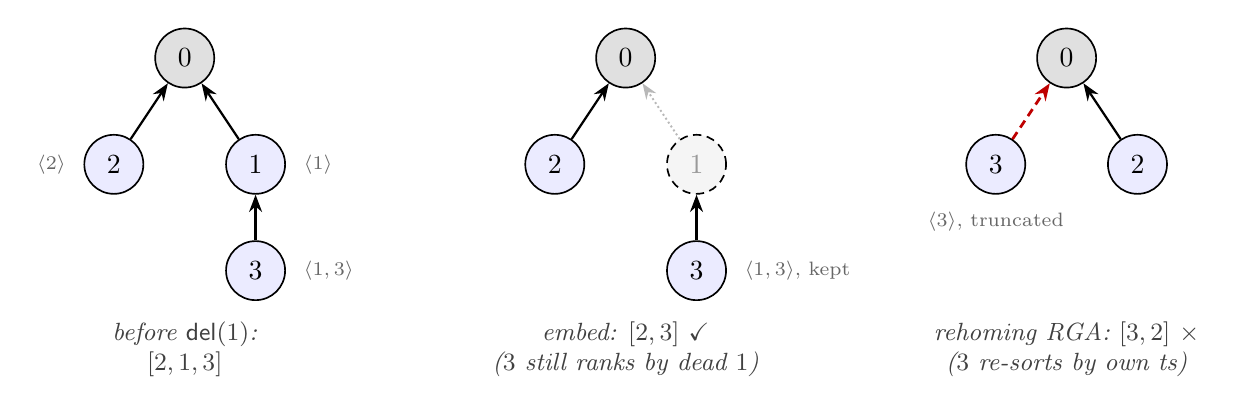
\begin{tikzpicture}
  % ---- before the delete: both designs agree
  \node[rootvtx] (br) at (0,0) {$0$};
  \node[vtx]  (b2) at (-0.9,-1.35) {$2$};
  \node[vtx]  (b1) at ( 0.9,-1.35) {$1$};
  \node[vtx]  (b3) at ( 0.9,-2.7)  {$3$};
  \draw[anc] (b2) -- (br);
  \draw[anc] (b1) -- (br);
  \draw[anc] (b3) -- (b1);
  \node[elbl, left=1mm of b2]  {$\langle 2\rangle$};
  \node[elbl, right=1mm of b1] {$\langle 1\rangle$};
  \node[elbl, right=1mm of b3] {$\langle 1,3\rangle$};
  \node[capt, align=center] at (0,-3.7)
    {before $\del(1)$:\\ $[2,1,3]$};
  % ---- embedded chain: key kept whole
  \begin{scope}[shift={(5.6,0)}]
  \node[rootvtx] (er) at (0,0) {$0$};
  \node[vtx]   (e2) at (-0.9,-1.35) {$2$};
  \node[deadv] (e1) at ( 0.9,-1.35) {$1$};
  \node[vtx]   (e3) at ( 0.9,-2.7)  {$3$};
  \draw[anc] (e2) -- (er);
  \draw[ghost] (e1) -- (er);
  \draw[anc] (e3) -- (e1);
  \node[elbl, right=1mm of e3] {$\langle 1,3\rangle$, kept};
  \node[capt, align=center] at (0,-3.7)
    {embed: $[2,3]$ \checkmark\\ ($3$ still ranks by dead $1$)};
  \end{scope}
  % ---- rehoming RGA: climb truncates the key
  \begin{scope}[shift={(11.2,0)}]
  \node[rootvtx] (fr) at (0,0) {$0$};
  \node[vtx] (f3) at (-0.9,-1.35) {$3$};
  \node[vtx] (f2) at ( 0.9,-1.35) {$2$};
  \draw[climb] (f3) -- (fr);
  \draw[anc]   (f2) -- (fr);
  \node[elbl, below=1mm of f3] {$\langle 3\rangle$, truncated};
  \node[capt, align=center] at (0,-3.7)
    {rehoming RGA: $[3,2]$ $\times$\\ ($3$ re-sorts by own ts)};
  \end{scope}
\end{tikzpicture}
\caption{The one-line separation on the L1 delete-reorder litmus:
insert $1$ and $2$ at the front, $3$ after $1$, delete $1$. The
rehoming RGA's climb (red) re-parents $3$ and re-sorts it by its \emph{own}
timestamp: the truncated key $\langle 3\rangle$ beats
$\langle 2\rangle$, and $3$ jumps over $2$. The embedded chain
$\langle 1,3\rangle$ keeps ranking $3$ by its dead parent's
timestamp: $[2,3]$, the delete-order-preserving read. Arrows point
from a node to its anchor; dashed grey = dead.}
\label{fig:l1}
\end{figure}

\paragraph{Worked example (Figure~\ref{fig:credential}).} $6$ and
$10$ concurrently insert at the
front: chains $\langle 6 \rangle$ and $\langle 10 \rangle$;
display $[10, 6]$, no arbitration, at every replica and merge order.
Type $22, 16$ under $6$: chains $\langle 6, 22 \rangle$,
$\langle 6, 16 \rangle$. Delete $6$: the records of $22$ and $16$ are
untouched and still carry $6$'s timestamp. A third party concurrently
inserts $8$ at the front: $\langle 8 \rangle$ sorts below
$\langle 10 \rangle$ and above $\langle 6, 22 \rangle$, so the display
is $[10, 8, 22, 16]$ whether $8$ arrives before or after $6$'s death
(machine-checked as the \emph{credential countermodel}, the shape that
kills every timestamp-oblivious variant, \S\ref{sec:validation}).

\begin{figure}[h]
\centering
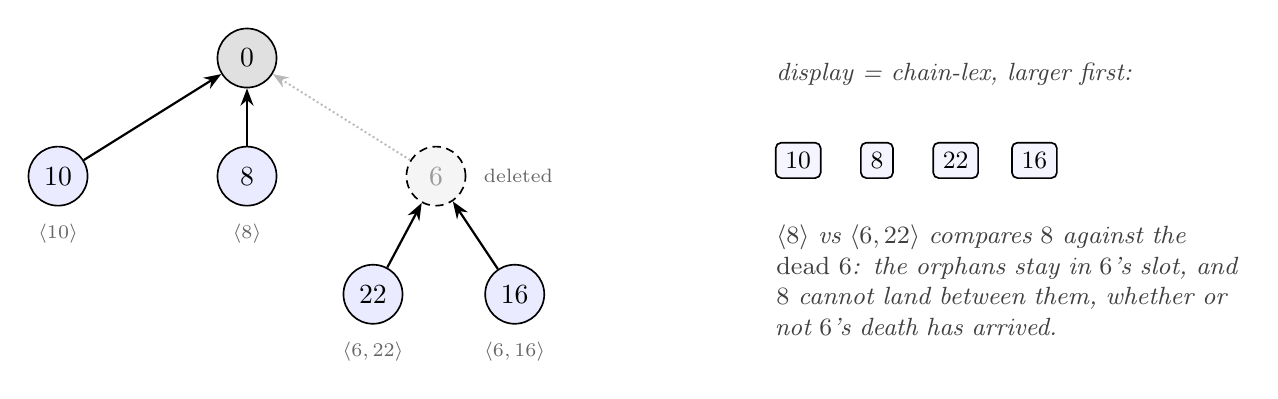
\begin{tikzpicture}
  \node[rootvtx] (r)   at (0,0)       {$0$};
  \node[vtx]     (n10) at (-2.4,-1.5) {$10$};
  \node[vtx]     (n8)  at (0,-1.5)    {$8$};
  \node[deadv]   (n6)  at (2.4,-1.5)  {$6$};
  \node[vtx]     (n22) at (1.6,-3.0)  {$22$};
  \node[vtx]     (n16) at (3.4,-3.0)  {$16$};
  \draw[anc]   (n10) -- (r);
  \draw[anc]   (n8)  -- (r);
  \draw[ghost] (n6)  -- (r);
  \draw[anc]   (n22) -- (n6);
  \draw[anc]   (n16) -- (n6);
  \node[elbl, below=1mm of n10] {$\langle 10\rangle$};
  \node[elbl, below=1mm of n8]  {$\langle 8\rangle$};
  \node[elbl, right=1mm of n6]  {deleted};
  \node[elbl, below=1mm of n22] {$\langle 6,22\rangle$};
  \node[elbl, below=1mm of n16] {$\langle 6,16\rangle$};
  \begin{scope}[shift={(7.0,-1.3)}]
    \node[capt, anchor=west] at (-0.4,1.1)
      {display = chain-lex, larger first:};
    \node[stbox] at (0,0)   {$10$};
    \node[stbox] at (1.0,0) {$8$};
    \node[stbox] at (2.0,0) {$22$};
    \node[stbox] at (3.0,0) {$16$};
    \node[capt, text width=5.9cm, align=left, anchor=north west]
      at (-0.4,-0.7)
      {$\langle 8\rangle$ vs $\langle 6,22\rangle$ compares $8$
       against the \emph{dead} $6$: the orphans stay in $6$'s slot,
       and $8$ cannot land between them, whether or not $6$'s
       death has arrived.};
  \end{scope}
\end{tikzpicture}
\caption{The credential countermodel as a birth tree. $6$ and $10$
race at the front; $22, 16$ are typed under $6$; $6$ dies; $8$
arrives at the front concurrently. Survivors sort by whole birth
chains, so the read is $[10,8,22,16]$ at every replica and merge
order. Every timestamp-oblivious variant flips this shape
(\S\ref{sec:related}).}
\label{fig:credential}
\end{figure}

\section{The representation: chains as entropy-coded coordinates}
\label{sec:encoding}

Everything above is the datatype; everything below is bits. A naive
carrier would store a full timestamp at every chain level (each
$\sim\!\log(\text{document age})$ bits, even for purely sequential
typing) and compare whole chains at every read. This section stores
the chains compactly without disturbing their order.

\paragraph{Vocabulary.} A \emph{codeword} is the bit string
$C(\delta)$ encoding one chain level: one element's timestamp,
stored as its differential $\delta$ to its birth anchor (step 1
below). A \emph{coordinate} is the bit string encoding a whole
chain: the concatenation, root to element, of one block per level
(the level's codeword plus three framing bits fixed by the mint
construction below), with nothing else marking the boundaries. We
write $|s|$ for the length in bits of a bit string $s$. Read as a
binary fraction, a coordinate names a dyadic interval in $(0,1)$;
codeword concatenation becomes interval nesting, and the interval is
the $\alpha(u)$ of Theorem~\ref{thm:faithful}. Bit string and
interval are two views of one object; we use whichever is clearer.

\paragraph{What the coding is for.} Two jobs, only one of which is
about correctness.
\emph{Job 1: cost.} The datatype layer already forced sort keys to
retain dead ancestors' timestamps (the conservation law,
\S\ref{sec:design}); the only remaining question is how many bits
that retention costs. Without entropy coding, ``tombstone-free''
would be bookkeeping: a full timestamp per level grows with document
age however calm the history. The \emph{unary control}
(\code{embed-tree}: the identical datatype with a unary code in the
mint, codeword length linear in the value, kept as the experiment's
cost-control arm; step 2 and the entropy-law table) makes the gap
measurable: 61\,KB against the coded design's 0.5\,KB on the table's
1000-element chain scenario. The coding is what makes
the headline claim true: the dead survive as the entropy of the
anchor gaps they were born across, and not more.
\emph{Job 2: faithfulness.} The chains must be stored so that plain
lexicographic bit comparison reproduces chain-lex exactly, in every
reachable state, forever. This is the single obligation the
representation owes \S\ref{sec:design}
(Theorem~\ref{thm:faithful}). Correctness lives upstairs; this layer
is an implementation that must not lie. Job 2 needs no entropy
optimality at all: it needs exactly two structural properties of the
per-level code, stated next.

\paragraph{The contract.} The stored form must support four
operations: \emph{mint} (insert: produce the new codeword from the
two timestamps alone, coordination-free, reading no siblings);
\emph{compare} (read: plain lexicographic comparison, with no tie
rule); \emph{fold} (delete: splice a dead node out by concatenating
its block into each child's stored string, exactly); and
\emph{refold} (merge: recompute survivors' coordinates by the same
concatenation). Each guarantee is bought by a specific property of
$C$:
\begin{itemize}
\item \textbf{Monotone} ($\delta < \delta' \Rightarrow C(\delta)
<_{\mathrm{lex}} C(\delta')$) buys correct \emph{compare}. A
chain-lex first difference always compares two same-anchor entries,
where timestamp order and $\delta$ order coincide (step 1); bitwise
comparison of coordinates therefore equals timestamp comparison at
the first differing level precisely when $C$ is monotone.
\item \textbf{Prefix-free} (no codeword is a prefix of another) buys
three things at once. \emph{Alignment}: in a comparison of two
coordinates, the first differing bit falls inside the first
differing level's codewords, so levels cannot be confused across
boundaries and no delimiters are needed; this is also what keeps
\emph{fold} and \emph{refold} exact splices. \emph{Geometry}: by the
Kraft correspondence, prefix-free codewords occupy pairwise-disjoint
dyadic cells, which is Theorem~\ref{thm:faithful}(i) and the reason
a concurrent front-insert can never land inside a dead sibling's
span (Figure~\ref{fig:nest}). \emph{No ties}: cell disjointness plus
Lamport uniqueness means sibling coordinates never tie, so the merge
never decides an order and the read needs no tiebreak.
\item \textbf{Universal, with a cheap floor} buys Job 1: $C$ is
defined for every $\delta \ge 1$, $|C(1)| = O(1)$ so continuation
typing costs a constant per level, and $|C(\delta)| = \Theta(\log
\delta)$ so a level pays the log of its anchor gap, whether the gap
is a race or a cursor jump (step 1), and nothing else.
\end{itemize}
Monotone plus prefix-free is all of Job 2: any such code satisfies
Theorem~\ref{thm:faithful}, which is why the Lean capstone is
parametric in the code (\S\ref{sec:mechanization}) and why the unary
control proves the same theorems at absurd cost. Entropy coding
enters only in \emph{which} monotone prefix-free code is chosen; the
choice sets the constant in the bits-per-level bill and nothing in
the correctness story. One requirement cuts across all four
operations: the arithmetic is exact, never rounded (see the binary64
refutation below).

\paragraph{Step 1: differential coding.} By causality
$\delta = x - a \ge 1$. A chain-lex first difference always compares
two entries with the \emph{same} anchor (the shared prefix), and for
a fixed anchor, ordering by $x$ and by $\delta$ coincide, so each
chain level may store the differential instead of the timestamp.
Call $\delta$ the \emph{anchor gap}: the events elapsed between the
anchor's mint and the insert's.
Continuation typing (each character anchored at its predecessor) has
$\delta = 1$ at every level regardless of how long the document has
lived. Two things widen the gap, and they pay the same bill: a
genuine race with timestamp gap $g$ costs $\log_2 g$ bits, and so
does a \emph{cursor jump}, the first character typed at an old
anchor; its successors anchor at fresh characters and are back to
$\delta = 1$. The differential is an encoding choice, not
semantics: the mathematical object remains the timestamp.

\paragraph{Step 2: entropy coding.} For $\delta \ge 1$ let $L$ be the
bit-length of $\delta$ and
\[
  C(\delta) \;=\; \underbrace{1\cdots1}_{L-1}\;0\;\bigl(\delta
  \text{ with its leading bit removed}\bigr)
  \qquad (|C(\delta)| = 2L-1),
\]
an order-preserving prefix-free code: exactly the contract. The
length accounting: prefix-freedom makes each codeword
self-delimiting, and a self-delimiting code over unbounded $\delta$
must spend bits twice, once on the value and once announcing its own
length. $C$ pays each bill at $\sim\!\log_2\delta$. The header
$1^{L-1}0$ is a unary announcement ``$L{-}1$ payload bits follow''
($L$ bits); the payload is $\delta$'s trailing $L{-}1$ bits, since
the leading bit of an $L$-bit number is always $1$: once the header
has said $L$ it carries no information and is dropped. Hence
\[
  |C(\delta)| \;=\; \underbrace{(L{-}1) + 1}_{\text{header}}
  \;+\; \underbrace{(L{-}1)}_{\text{payload}}
  \;=\; 2L - 1 \;=\; 2\lfloor \log_2 \delta \rfloor + 1,
\]
e.g.\ $C(1) = 0$, $C(2) = 100$, $C(3) = 101$, $C(5) = 11001$. This
is Elias~$\gamma$ with
its header flipped: $\gamma$ announces the length in \emph{zeros},
which is prefix-free but order-reversing across length classes:
at the first divergence the longer, hence larger, number shows a
header $0$ against the shorter's leading payload bit $1$. Writing
the header in ones makes that same position decide in favor of the
longer code, so lexicographic order on codewords is numeric order on
$\delta$. The $\gamma$-flip is the building block, not the last
word: only the \emph{value} bill is forced at $\log_2 \delta$, and
the \emph{length} bill can itself be entropy-coded. Applying $C$ to
the length field (then the payload) gives the order-preserving flip
of \textbf{Elias~$\delta$}, prefix-free and monotone by the same
across-length-class argument, at $\log_2 \delta + O(\log \log
\delta)$ per level; \emph{this is the canonical mint}.
\emph{Any} order-preserving prefix-free
code works here, and the artifact exists in three proved encodings
of one datatype (\code{embed-tree} unary, \code{embed-code} the
$\gamma$-flip, \code{eliasDeltaCode} the $\delta$-flip); the capstone
theorem is inherited at each verbatim, with zero new proof content
(\S\ref{sec:mechanization}): the code-parametricity claim,
machine-validated. Two honest footnotes: per level the $\delta$-flip
wins only from $\delta \ge 32$ and loses at $\delta \in \{2,3\} \cup
[8,15]$ (kernel-checked length comparisons), and measured editing
tails are thin, so on real traces the two flips are a wash; the
dominance shows in race-heavy shapes (the entropy-law table below)
and in the asymptotics.

\paragraph{The mint.} Writing $b = 1 \cdot C(\delta)$ (a leading 1
keeps coordinates positive) and $w = 2^{-|b|-2}$, the mint is the
second quarter of $b$'s dyadic cell:
\[
  M(\delta) \;=\; \bigl(\,0.b + w,\ \ 0.b + 2w\,\bigr)
  \;\subset\; \bigl[\,0.b,\ 0.b + 4w\,\bigr) .
\]
The quarter placement leaves a gap below and headroom above inside the
cell, and the open space $(0.b+2w,\, 0.b+4w)$ is never minted: it
exists so that the interval has room to \emph{contain} the node's own
subtree without touching the next cell. This also pins down the
per-level \emph{block} promised in the vocabulary: $0.b + w$ written
as a string is $b\,\code{01}$, so the block is
$1\,C(\delta)\,\code{01}$, the codeword in its three framing bits
(the leading $1$ for positivity, the \code{01} that selects the
second quarter). The block is what a node stores; read as a binary
fraction it is the lower endpoint of $M(\delta)$, and flipping the
trailing \code{01} to \code{10} gives the upper. Worked out for
small deltas:

\begin{center}\small
\begin{tabular}{@{}rllll@{}}
\toprule
$\delta$ & $C(\delta)$ & block $= 1\,C(\delta)\,\code{01}$ &
  $M(\delta)$ & bits/level \\
\midrule
1   & \code{0}             & \code{1001}     & $(9/16,\ 10/16)$   & 4 \\
2   & \code{100}           & \code{110001}   & $(49/64,\ 50/64)$  & 6 \\
3   & \code{101}           & \code{110101}   & $(53/64,\ 54/64)$  & 6 \\
4   & \code{11000}         & \code{11100001} & $(225/256,\ 226/256)$ & 8 \\
5   & \code{11001}         & \code{11100101} & $(229/256,\ 230/256)$ & 8 \\
10  & \code{1110010}       & \code{1111001001} & $(969/1024,\ 970/1024)$ & 10 \\
100 & \code{1111110100100} & \code{1111111010010001} &
  $(65169/65536,\ 65170/65536)$ & 16 \\
\bottomrule
\end{tabular}
\end{center}

\noindent Three things to read off. The endpoints are consecutive
dyadics at scale $2^{-(|b|+2)}$ (numerators $n$ and $n{+}1$): the
mint is one tick wide at its own scale, with the tick below it (the
gap) and the two ticks above it (the subtree headroom) never minted.
The rows are strictly increasing as fractions: monotonicity made
visible. And the bit count is $2L + 2$ for an $L$-bit $\delta$: four
bits at $\delta = 1$ (the sequential-typing constant of the entropy
law), sixteen at $\delta = 100$.

\begin{figure}[h]
\centering
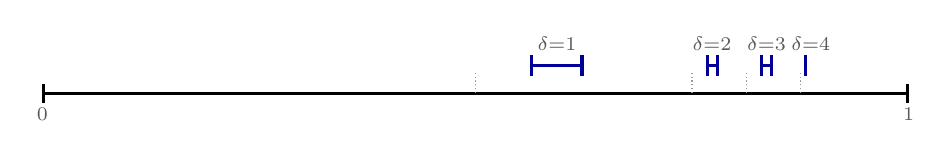
\begin{tikzpicture}[xscale=11]
  \draw[rng] (0,0) -- (1,0);
  \node[lab, below] at (0,-0.06) {$0$};
  \node[lab, below] at (1,-0.06) {$1$};
  % cells for delta = 1..4 : b = 1C(d); mint = (0.b + w, 0.b + 2w), w = 2^-(|b|+2)
  % d=1: C='0', b='10'  cell [1/2, 3/4)        mint (0.5625, 0.625)
  % d=2: C='100', b='1100' cell [3/4, 13/16)   mint (0.765625, 0.78125)
  % d=3: C='101', b='1101' cell [13/16, 7/8)   mint (0.828125, 0.84375)
  % d=4: C='11000', b='111000' cell [7/8, 57/64) mint (0.87890625, 0.8828125)
  \draw[rngB] (0.5625,0.35) -- (0.625,0.35);
  \node[lab, above] at (0.594,0.42) {$\delta{=}1$};
  \draw[rngB] (0.765625,0.35) -- (0.78125,0.35);
  \node[lab, above] at (0.773,0.42) {$\delta{=}2$};
  \draw[rngB] (0.828125,0.35) -- (0.84375,0.35);
  \node[lab, above] at (0.836,0.42) {$\delta{=}3$};
  \draw[rngB] (0.87890625,0.35) -- (0.8828125,0.35);
  \node[lab, above] at (0.887,0.42) {$\delta{=}4$};
  \draw[black!40, densely dotted] (0.5,0.0) -- (0.5,0.28);
  \draw[black!40, densely dotted] (0.75,0.0) -- (0.75,0.28);
  \draw[black!40, densely dotted] (0.8125,0.0) -- (0.8125,0.28);
  \draw[black!40, densely dotted] (0.875,0.0) -- (0.875,0.28);
\end{tikzpicture}
\caption{Mints $M(\delta)$ for $\delta = 1..4$ inside the parent's unit
interval (cell boundaries dotted). Larger deltas sit strictly higher;
distinct deltas are disjoint with gaps; each mint is a quarter of its
cell, leaving room for the node's own subtree. Drawn for the
$\gamma$-flip $C$; the construction reads verbatim over any
order-preserving prefix-free code, in particular the canonical
Elias-$\delta$ mint (step 2).}
\label{fig:mint}
\end{figure}

\paragraph{The stored state.} The carrier stores each live node
parent-relatively:
\[
  \sigma \;:\; t \;\mapsto\; (\,\mathrm{par} \in \mathbb{N},\ \
  s \in \{0,1\}^{*},\ \ \mathrm{char}\,),
\]
where $s$ is a block ($1\,C(\delta)\,\code{01}$ at birth; after
folds, below, a concatenation of blocks) \emph{relative to the
parent}, and $\mathrm{par} = 0$ denotes the root sentinel (which
owns $(0,1)$ and is never stored). The record holds no interval; the
interval is the string's decoding,
\[
  (lo, hi) \;=\; \bigl(\,0.s,\ \ 0.s + 2^{-|s|}\,\bigr)
  \;\subset\; (0,1),
\]
consecutive dyadics at $s$'s own scale, one block at a time exactly
as in the mint table. The maintenance below and
Theorem~\ref{thm:faithful} are stated on the intervals, and every
operation they perform on an interval is a string operation on $s$:
composition is concatenation, comparison is lexicographic. (The
validation model stores the decoded pair directly, as exact
fractions.) A node's \emph{absolute} interval is the affine
composition of the intervals along its parent chain. For a node $v$
with mint $M(\delta_v) = (lo_v,\ lo_v + w_v)$, let
\[
  \varphi_v : (0,1) \to M(\delta_v), \qquad
  \varphi_v(x) \;=\; lo_v + w_v \cdot x,
\]
the unique increasing affine bijection of the unit interval onto
$v$'s mint; it maps a subinterval $(a,b)$ to
$(lo_v + w_v a,\ lo_v + w_v b)$, and on strings it prefixes $v$'s
block: $\varphi_v(0.y) = 0.(s_v\, y)$. Write
\[
  \alpha(u) \;=\; \varphi_{c_1} \circ \cdots \circ
  \varphi_{c_k}\bigl(M(\delta_u)\bigr)
\]
for the composition along $u$'s birth chain $c_1 \cdots c_k\,u$
($\delta_v$ is $v$'s delta to its birth parent): $\alpha(u)$ is the
\emph{encoding of $\chain(u)$}, and at the string level it decodes
the concatenation of the blocks along the chain. Worked on the tree
of Figure~\ref{fig:credential}, redrawn before $\del(6)$ with the
delta (child minus anchor) on each edge and the stored block under
each node:

\begin{center}
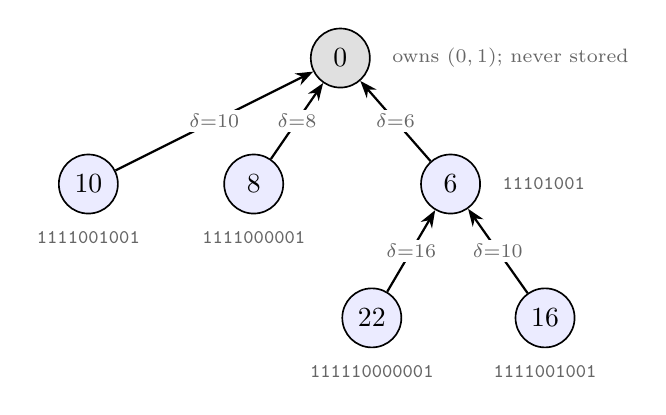
\begin{tikzpicture}
  \node[rootvtx] (r)   at (0,0)        {$0$};
  \node[elbl, right=1.5mm of r] {owns $(0,1)$; never stored};
  \node[vtx] (n10) at (-3.2,-1.6) {$10$};
  \node[vtx] (n8)  at (-1.1,-1.6) {$8$};
  \node[vtx] (n6)  at (1.4,-1.6)  {$6$};
  \node[vtx] (n22) at (0.4,-3.3)  {$22$};
  \node[vtx] (n16) at (2.6,-3.3)  {$16$};
  \draw[anc] (n10) -- (r)
    node[elbl, midway, fill=white, inner sep=1.5pt] {$\delta{=}10$};
  \draw[anc] (n8) -- (r)
    node[elbl, midway, fill=white, inner sep=1.5pt] {$\delta{=}8$};
  \draw[anc] (n6) -- (r)
    node[elbl, midway, fill=white, inner sep=1.5pt] {$\delta{=}6$};
  \draw[anc] (n22) -- (n6)
    node[elbl, midway, fill=white, inner sep=1.5pt] {$\delta{=}16$};
  \draw[anc] (n16) -- (n6)
    node[elbl, midway, fill=white, inner sep=1.5pt] {$\delta{=}10$};
  \node[elbl, below=1mm of n10] {\code{1111001001}};
  \node[elbl, below=1mm of n8]  {\code{1111000001}};
  \node[elbl, right=1.5mm of n6] {\code{11101001}};
  \node[elbl, below=1mm of n22] {\code{111110000001}};
  \node[elbl, below=1mm of n16] {\code{1111001001}};
\end{tikzpicture}
\end{center}

\noindent Writing $(n, n{+}1)/2^{k}$ for the interval
$(n/2^k,\ (n{+}1)/2^k)$ and $\approx$ for its lower endpoint:

\begin{center}\small
\setlength{\tabcolsep}{4.5pt}
\begin{tabular}{@{}rrllll@{}}
\toprule
node & $\delta$ & stores $(\mathrm{par}, s)$ & decode of $s$ &
  $\alpha$ (absolute) & $\approx$ \\
\midrule
$10$ & $10$ & $(0,\ \code{1111001001})$   & $(969, 970)/2^{10}$ &
  $(969, 970)/2^{10}$ & $0.94629$ \\
$8$  & $8$  & $(0,\ \code{1111000001})$   & $(961, 962)/2^{10}$ &
  $(961, 962)/2^{10}$ & $0.93848$ \\
$6$  & $6$  & $(0,\ \code{11101001})$     & $(233, 234)/2^{8}$  &
  $(233, 234)/2^{8}$  & $0.91016$ \\
$22$ & $16$ & $(6,\ \code{111110000001})$ & $(3969, 3970)/2^{12}$ &
  $(958337, 958338)/2^{20}$ & $0.91394$ \\
$16$ & $10$ & $(6,\ \code{1111001001})$   & $(969, 970)/2^{10}$ &
  $(239561, 239562)/2^{18}$ & $0.91385$ \\
\bottomrule
\end{tabular}
\end{center}

\noindent The root's children store their absolute intervals already
($\mathrm{par} = 0$). The grandchildren compose: $22$'s absolute
string is its parent's block followed by its own,
$\code{11101001}\,\code{111110000001}$ ($20$ bits, hence the
$2^{20}$), and likewise $16$'s ($18$ bits). Both absolute intervals
sit inside $M(6) = (0.91016, 0.91406)$ while $8$'s sits above it, so
the descending-$\alpha$ read is $[10, 8, 22, 16]$ and $8$ cannot
land between the orphans. Nodes $16$ and $10$ store the same
string, both being $\delta = 10$ births; records are
parent-relative, so this is no collision. After $\del(6)$ the fold
rewrites the two records to $(\mathrm{par}\ 0,\ \text{the
concatenated } s)$ and the $\alpha$ column is unchanged bit for bit.
Figure~\ref{fig:nest} draws these intervals (widths schematic).

\begin{figure}[h]
\centering
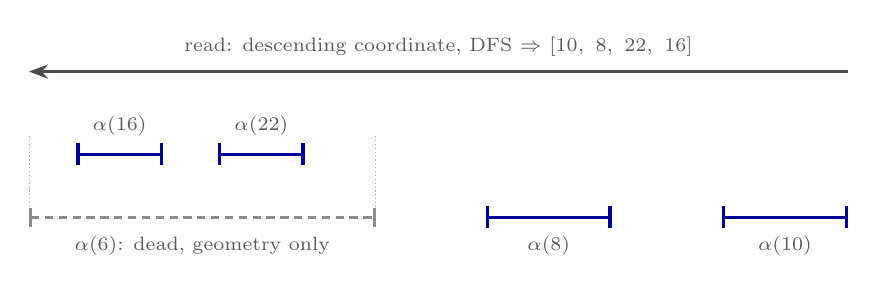
\begin{tikzpicture}
  % depth-1 intervals (schematic widths; true mints are dyadic, Fig 1)
  \draw[rngD] (0.6,0) -- (5.0,0);
  \node[lab, below] at (2.8,-0.12) {$\alpha(6)$: dead, geometry only};
  \draw[rngB] (6.4,0) -- (8.0,0);
  \node[lab, below] at (7.2,-0.12) {$\alpha(8)$};
  \draw[rngB] (9.4,0) -- (11.0,0);
  \node[lab, below] at (10.2,-0.12) {$\alpha(10)$};
  % depth-2 mints, nested inside alpha(6)
  \draw[rngB] (1.2,0.8) -- (2.3,0.8);
  \node[lab, above] at (1.75,0.92) {$\alpha(16)$};
  \draw[rngB] (3.0,0.8) -- (4.1,0.8);
  \node[lab, above] at (3.55,0.92) {$\alpha(22)$};
  \draw[black!35, densely dotted] (0.6,0.08) -- (0.6,1.05);
  \draw[black!35, densely dotted] (5.0,0.08) -- (5.0,1.05);
  % read direction
  \draw[-{Stealth[length=2.4mm]}, line width=0.9pt, black!70]
    (11.0,1.85) -- (0.6,1.85);
  \node[lab, above] at (5.8,1.92)
    {read: descending coordinate, DFS $\Rightarrow$ $[10,\ 8,\ 22,\ 16]$};
\end{tikzpicture}
\caption{Figure~\ref{fig:credential} downstairs (widths schematic;
true mints are the dyadic cells of Figure~\ref{fig:mint}). Deleting
$6$ removes its record, but $\alpha(16)$ and $\alpha(22)$ are
compositions \emph{through} $M(6)$: the dead node survives as the
dashed container, the tombstone compressed into geometry. $8$'s
interval can never land inside $\alpha(6)$'s span: distinct deltas
occupy disjoint cells (Theorem~\ref{thm:faithful}(i)), which is the
credential verdict, now a fact about intervals.}
\label{fig:nest}
\end{figure}

\paragraph{Maintenance.} How the stored form tracks the datatype:
\begin{itemize}
\item $\ins(x \leftarrow a)$ mints $M(x - a)$ relative to $a$: the
new record depends only on the two timestamps.
\item $\del(d)$ \emph{isometrically folds} $d$ into its children:
each child $c$ is re-parented to $d$'s parent and $d$'s record is
substituted into $c$'s. On the stored strings this is concatenation,
$c.s := d.s\, c.s$; read as intervals, $c.\mathrm{frac} :=
d.\mathrm{frac} \circ c.\mathrm{frac}$, where $I \circ J$ is the
image of $J$ under the increasing affine bijection of $(0,1)$ onto
$I$ (the $\varphi$ of the stored state, with $I$ in place of a
mint): for $I = (lo,\ lo + w)$,
\[
  I \circ J \;=\; (\,lo + w \cdot lo_J,\ \ lo + w \cdot hi_J\,).
\]
The substitution is exact. Upstairs, deletion
changes nobody's sort key (\S\ref{sec:design}); the fold is the
parent-relative storage scheme \emph{re-normalizing} while every
absolute interval stays fixed (Figure~\ref{fig:fold}):
representation maintenance, not datatype semantics. On the running
example, $\del(6)$ removes $6$'s record and substitutes it into both
children: $22$'s record $(6,\ \code{111110000001})$ becomes
$(0,\ \code{11101001}\,\code{111110000001})$, whose decode is
\[
  (233, 234)/2^{8} \circ (3969, 3970)/2^{12}
  \;=\; (233 \cdot 2^{12} + 3969,\ 233 \cdot 2^{12} + 3970)/2^{20}
  \;=\; (958337, 958338)/2^{20},
\]
and likewise $16$'s becomes $(0,\
\code{11101001}\,\code{1111001001})$, decoding $(239561,
239562)/2^{18}$. Both are exactly the $\alpha$ column of the worked
table: the absolute intervals did not move, only the
parent-relative bookkeeping did.
\item The merge \emph{refolds}: for each survivor, compute its
absolute interval by folding its record to the root inside the input
that holds it (a record's stored parent is always live in its own
input, so the chain stays in one input; by
Theorem~\ref{thm:faithful}(iii) the choice of input cannot matter,
asserted at runtime and never fired); re-parent to the nearest
\emph{surviving} ancestor; re-relativize.
\item The read is depth-first from the root, children in descending
order of $lo$. No tie rule is needed (Corollary~\ref{cor:lex}).
\end{itemize}

\begin{figure}[h]
\centering
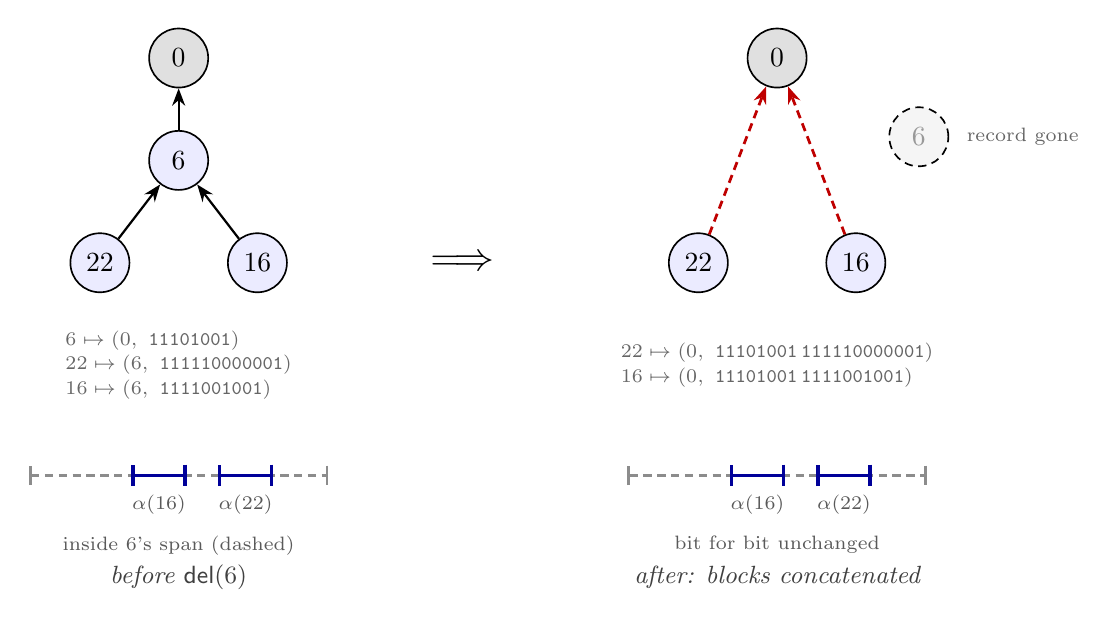
\begin{tikzpicture}
  % ---- before del(6): parent-relative records
  \node[rootvtx] (ar)  at (0,0)     {$0$};
  \node[vtx]     (a6)  at (0,-1.3)  {$6$};
  \node[vtx]     (a22) at (-1.0,-2.6) {$22$};
  \node[vtx]     (a16) at ( 1.0,-2.6) {$16$};
  \draw[anc] (a6)  -- (ar);
  \draw[anc] (a22) -- (a6);
  \draw[anc] (a16) -- (a6);
  \node[elbl, align=left] at (0,-3.9)
    {$6  \mapsto (0,\ \code{11101001})$\\[1pt]
     $22 \mapsto (6,\ \code{111110000001})$\\[1pt]
     $16 \mapsto (6,\ \code{1111001001})$};
  \draw[rngD] (-1.9,-5.3) -- (1.9,-5.3);
  \draw[rngB] (-0.6,-5.3) -- (0.1,-5.3);
  \draw[rngB] ( 0.5,-5.3) -- (1.2,-5.3);
  \node[lab, below] at (-0.25,-5.42) {$\alpha(16)$};
  \node[lab, below] at ( 0.85,-5.42) {$\alpha(22)$};
  \node[lab, below] at (0,-5.95) {inside $6$'s span (dashed)};
  \node[capt] at (0,-6.6) {before $\del(6)$};
  % ---- arrow
  \node at (3.6,-2.6) {\Large $\Longrightarrow$};
  % ---- after: blocks concatenated, absolute intervals fixed
  \begin{scope}[shift={(7.6,0)}]
  \node[rootvtx] (br)  at (0,0)     {$0$};
  \node[deadv]   (b6)  at (1.8,-1.0) {$6$};
  \node[elbl, right=1mm of b6] {record gone};
  \node[vtx]     (b22) at (-1.0,-2.6) {$22$};
  \node[vtx]     (b16) at ( 1.0,-2.6) {$16$};
  \draw[climb] (b22) -- (br);
  \draw[climb] (b16) -- (br);
  \node[elbl, align=left] at (0,-3.9)
    {$22 \mapsto (0,\ \code{11101001}\,\code{111110000001})$\\[1pt]
     $16 \mapsto (0,\ \code{11101001}\,\code{1111001001})$};
  \draw[rngD] (-1.9,-5.3) -- (1.9,-5.3);
  \draw[rngB] (-0.6,-5.3) -- (0.1,-5.3);
  \draw[rngB] ( 0.5,-5.3) -- (1.2,-5.3);
  \node[lab, below] at (-0.25,-5.42) {$\alpha(16)$};
  \node[lab, below] at ( 0.85,-5.42) {$\alpha(22)$};
  \node[lab, below] at (0,-5.95) {bit for bit unchanged};
  \node[capt] at (0,-6.6) {after: blocks concatenated};
  \end{scope}
\end{tikzpicture}
\caption{The isometric fold on the running example. $\del(6)$
deletes $6$'s record and concatenates its block \code{11101001}
onto the front of each child's, re-parenting both to the root (red:
the re-parenting, a storage move only). The stored states change:
$22$ and $16$ now carry two-block strings and $\mathrm{par}\ 0$.
The absolute intervals $\alpha(22) = (958337, 958338)/2^{20}$ and
$\alpha(16) = (239561, 239562)/2^{18}$, and with them the display,
are bit-for-bit unchanged: upstairs, the sort keys still read
$\langle 6, 22\rangle$ and $\langle 6, 16\rangle$. The dashed span
is $6$'s old interval, surviving as pure geometry.}
\label{fig:fold}
\end{figure}

\paragraph{Why the codeword must announce its own end.} Before the
theorem, the countermodel that motivates it. A single codeword in a
field of known extent needs no header, and the length looks
recoverable from the string itself; plain binary shows what breaks,
once per purchase in the contract. \emph{Geometry:} $B(2) = \code{10}$
prefixes $B(5) = \code{101}$, so $B(5)$'s cell sits inside $B(2)$'s;
containment means ancestry, so the $\delta{=}5$ sibling lands amid
the $\delta{=}2$ sibling's descendants and non-interleaving dies
with everything alive. \emph{Parsing:} once a fold erases the
structural boundary between blocks, \code{101100\ldots} reads as
$B(2)$ then \code{11\ldots} or as $B(5)$ then \code{00\ldots}, and
nothing outside the string can say. \emph{Ties:} a binary fraction
cannot see trailing zeros, so \code{10} and \code{100} both denote
$\tfrac12$; distinct siblings mint touching intervals, and the id
tiebreak wakes into an arbiter that orders by id, not chain-lex.
Nor can the header bits be dodged: prefix-freedom demands
$\sum_\delta 2^{-\ell(\delta)} \le 1$, and plain binary puts
$2^{L-1}$ values at every length $L$, so every prefix-free code
pays a length announcement of order $\log L$ somewhere (out-of-band
boundary tables cost the same bits and forfeit the string as a
self-contained key; database key encodings inline it for the same
reason). And the fold names where the boundary went: the tree node
that carried it structurally is the deleted tombstone, whose
ordering verdict becomes the payload and whose boundary becomes the
header. ``Tombstone compressed into coordinate entropy'' is literal
at the bit level.

\paragraph{The one obligation.} The four theorems of the earlier
drafts collapse into a single statement about the encoding.

\begin{theorem}[encoding faithfulness]\label{thm:faithful}
\begin{itemize}
\item[(i)] \emph{Order-embedding at one level:} for $\delta \ne
\delta'$, $M(\delta)$ and $M(\delta')$ are disjoint with a gap;
$\delta < \delta' \Rightarrow M(\delta)$ lies entirely below
$M(\delta')$.
\item[(ii)] \emph{Homomorphism:} $\alpha$ realizes chain
concatenation as affine composition and embeds chain-lex in the
interval order: for distinct $u, v$, if $\chain(u)$ is a proper
prefix of $\chain(v)$ then $\alpha(v) \subset \alpha(u)$ (and, if
both are live, the two are never read-time siblings); otherwise
$\alpha(u) \cap \alpha(v) = \varnothing$, with the chain-lex-greater
element's interval strictly higher.
\item[(iii)] \emph{Exact maintenance:} in every reachable state,
every live node's stored records compose to exactly $\alpha(u)$.
\end{itemize}
\end{theorem}
\begin{proof}
(i) $C$ is prefix-free: codes of lengths $2L{-}1 < 2M{-}1$ differ at
position $L$ (the shorter's header terminator $0$ against the longer's
header $1$); equal-length codes differ in the payload. Prefix-free
codes have pairwise-disjoint dyadic cells. $C$ is monotone as a binary
fraction: within a length class the payload is $\delta$'s low bits in
order; across classes the position-$L$ bit decides in favor of the
longer code. Disjoint cells ordered by their codes, and mints interior
quarters of their cells, give both claims.
(ii) If neither chain is a prefix of the other, they first differ on
distinct deltas relative to the \emph{same} birth ancestor
(\S\ref{sec:encoding}, step 1); (i) separates them there, and affine
images of disjoint intervals are disjoint and order-preserved (each
$\varphi$ is increasing). If $\chain(u)$ prefixes $\chain(v)$, then
$\alpha(v) \subseteq \varphi_{c_1} \circ \cdots \circ
\varphi_{c_k}(\varphi_u((0,1))) = \alpha(u)$ by construction; and if
both are live, $v$'s nearest live ancestor is $u$ or deeper, so
they never share a current parent, and sibling groups are pairwise
disjoint.
(iii) By induction over transitions. $\ins$ establishes it by
definition. $\del$'s fold replaces $(\mathrm{par}, \mathrm{frac})$
pairs by their exact composition, leaving $\alpha$ unchanged. The merge
recomputes precisely $\alpha(u)$ (folding a record chain to the root)
and re-relativizes against another $\alpha$; ties cannot exist by
(i) and (ii), so no step of any transition ever rewrites an interval
by anything but exact composition.
\end{proof}

\begin{corollary}[display $\equiv$ chain-lex; no tie rule]
\label{cor:lex}
The read (DFS by descending $lo$) enumerates survivors in exactly
chain-lex order: per level, larger delta first, so among same-parent
siblings, exactly newest first; survivors rank by their own
timestamps, folded heirs by their dead founder's. Sibling $lo$-values
never tie; the read's id tiebreak is dead code. Machine checks:
pairwise sibling disjointness asserted at every read of $320$
randomized executions, all clean; over $19{,}531$ multi-member sibling
groups, own-timestamp order violated $3{,}481$ times (exactly the
post-fold heir groups; forcing own-ts there is the refuted
dissolution behavior), \textbf{chain-lex violated $0$ times}.
\end{corollary}

\paragraph{The entropy law.} A coordinate is the concatenation of the
codes along the birth chain: $\Theta(\sum_i \log \delta_i)$ bits,
the entropy of the chain. Continuation typing ($\delta = 1$ at every
level) costs $\sim$4 bits per level under every code here; a level
minted across an event gap $g$, by a race or by the first character
after a cursor jump, costs $\log_2 g + O(\log \log g)$ bits under
the canonical Elias-$\delta$ mint ($2\log_2 g + 1$ under the
$\gamma$-flip). \emph{The state pays for the magnitude of edit
non-locality, concurrent or not, and for nothing else.} Measured (1000
elements; the numbers are \emph{order metadata alone}, survivors'
coordinate bits read off the dyadic denominators; characters are
excluded, since data costs are identical across all designs):

\begin{center}\small
\setlength{\tabcolsep}{4.5pt}
\begin{tabular}{@{}lcccc@{}}
\toprule
scenario & \shortstack[c]{quarter carve\\ (refuted)} &
  unary mint & $\gamma$-flip mint & \textbf{Elias-$\delta$ mint} \\
\midrule
chain then delete-all ($\delta{=}1$) & $2^{2001}$ &
  $2^{502501}$ ($\sim$61 KB) & $2^{4001}$ ($\sim$0.5 KB) &
  $\boldsymbol{2^{4001}}$ ($\sim$0.5 KB) \\
1000 root siblings ($\delta{=}t$) & --- (ties) &
  max $2^{1003}$, 125 KB & max $2^{23}$, 5 KB &
  \textbf{max $\boldsymbol{2^{20}}$, 4 KB} \\
\bottomrule
\end{tabular}
\end{center}

\paragraph{The carrier.} The natural representation is a
\textbf{parent-relative bit string per node}: the fold is
concatenation, comparison is lexicographic ($O(1)$-ish with
structure sharing); the rationals are the semantics of the strings,
kept for the proofs. Nothing here computes $M(\delta)$: the
endpoints $0.b + w$ and $0.b + 2w$ are the strings $b\,\code{01}$
and $b\,\code{10}$, so the mint emits a block and the fold
concatenates, and $hi$ need not be stored at all. The Lean
mechanization drops even the framing bits: its coordinate is the
bare codeword concatenation on \code{List Bool} (\code{mint} appends
$\Gamma.\mathrm{enc}(t - a)$ to the anchor's coordinate), with the
prefix rule stated directly on strings; the quarter framing serves
the interval realization alone, buying positivity and subtree
interiority. The rational $M(\delta)$ is computed in exactly one
place, the validation model \code{embed\_tree.py}, as exact
fractions; the entropy tables read their bit counts off those
denominators. IEEE 754 binary64 is machine-refuted as the
carrier, a faithfulness failure rather than a design failure: mints
degenerate at $t = 52$, depths underflow at 44, and rounding voids
Theorem~\ref{thm:faithful}(iii) (6/120 PBT executions die). The
obstruction is a pigeonhole (chains carry $\Theta(\sum \log
\delta)$ bits; a fixed-width word holds 64), but binary64 is sound
as a \emph{comparison cache} with exact fallback on float equality.

\paragraph{Timestamps in practice.} The unique stamps in
$\mathbb{N}^{+}$ are Lamport's 1978 construction, flattened: each
replica ticks a counter per local operation, advances it to the max
on merge, and breaks ties by replica id, packed as
$t \cdot 2^{k} + r$ with $k$ id bits. Uniqueness and causality
($t_a < t_x$ gives $\mathrm{packed}_a < \mathrm{packed}_x$ regardless
of ids, so $\delta \ge 1$) both survive the packing; the proof layer
only \emph{assumes} uniqueness (the Lamport-structural part of
honesty), and this construction is the witness that the assumption is
realizable. Two entropy caveats. \emph{(i)} Packing inflates every
delta by $2^{k}$, costing $\sim$$2k$ extra bits per chain level, which
turns the 0.5 KB sequential run above into $\sim$3 KB at $k = 10$.
Cheaper: extend the mint's code to the pair, $C(\Delta t)$ followed
by a $k$-bit id. The pair code is still order-preserving prefix-free
(lex on $(\Delta t, r)$), and costs $k$ bits only where the level is
minted. A further option, unvalidated against the battery and
recorded as a design note, is to order sibling ids \emph{relative to
the anchor's} (any deterministic per-anchor id order is a legitimate
tiebreak; convergence needs agreement, not a uniform order), making
``same author as my anchor'', i.e.\ sequential typing, cost $\sim$1
bit, so only genuine cross-author races pay $\log R$. \emph{(ii)} The
clock must be \emph{dense logical time, never physical}: wall-clock
or HLC stamps make $\delta$ measure elapsed time rather than elapsed
events: a keystroke every 100\,ms over $\mu$s-resolution stamps
mints $\delta \approx 10^{5}$, $\sim$34 bits per level for a purely
sequential edit. The entropy law holds precisely because the counter
ticks once per event, making $\delta$ an event-count gap; if
wall-clock order is ever wanted, it belongs in a display-layer
tiebreak, never in the minted coordinate.

\paragraph{What remains open.} Dead chain entries concatenated into
survivors' strings are the conservation law's irreducible content
(\S\ref{sec:design}); reclaiming them under \emph{causal stability}
(renumber once every replica has seen the delete, the only
condition under which rewriting geometry is safe, since no verdict
involving the dead can be contested again) is the deepest of the
open cost items, and it is orthogonal to correctness. The wider
compression headroom is catalogued with its research questions in
the companion assessment
\code{whiteboard/order-coding-compression-notes.md}:
context-conditioned per-anchor codes (licensed by comparison
locality: a chain-lex first difference never crosses anchors),
coalescing $\delta{=}1$ runs, Steiner-sharing dead prefixes across
co-heirs, stability-gated rank re-coding, and the Elias-$\delta$
constant (step 2 above).

\section{The insert prefix: for the proof, and the proof alone}
\label{sec:prefix}

The insert payload $\pi$ exists for verification, not execution.
This section says why it must exist, and why an implementation may
drop it from the wire.

\paragraph{Why $\rc$ must be \Either.} The verification framework
(\S\ref{sec:mechanization}) resolves a concurrent pair of
non-commuting operations by consulting a declared
conflict-resolution order $\rc$; any \emph{oriented} entry for an
insert/delete pair, however, incurs a base commutation obligation
that is machine-refuted for this design space: ordering
$\ins(x \leftarrow a)$ against $\del(a)$ (in either direction) is
undischargeable as a conflict entry, because rehoming is
non-transitive across chains of deletions. So $\rc = \Either$: the
proof must show the two \emph{commute}, in both orders, on all
applicable states.

\paragraph{The commutation, and where the prefix earns its keep.}
Order 1, $\ins(x \leftarrow a)$ then $\del(a)$: $x$ is born with
chain $\pi \cdot x$, and the delete touches no chain (downstairs: the
fold re-homes $x$'s record with composed coordinates; by exactness
$\alpha(x) = \alpha(a) \circ M(x - a)$). Order 2, $\del(a)$ then
$\ins(x \leftarrow a)$: $a$ is gone; application must still be
\emph{total} and land $x$ on the same sort key. This is what the
carried prefix $\pi = \chain(a)$ (equivalently, the anchor's
coordinate) provides: apply sets
$\chain(x) = \pi \cdot x$ (downstairs:
$\alpha(x) = \pi \circ M(x - a)$, attached to the nearest live
ancestor). The two orders produce \emph{equal} states: commutation
to equality, not merely up to $\approx$, courtesy of canonicity
(Theorem~\ref{thm:chain}). Figure~\ref{fig:commute} draws the square
on the smallest instance.

\begin{figure}[h]
\centering
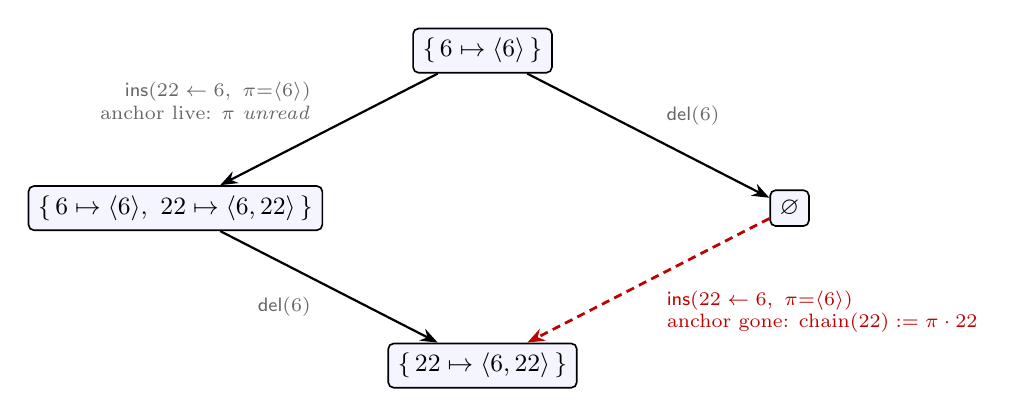
\begin{tikzpicture}
  \node[stbox] (s0) at (0,0)      {$\{\,6 \mapsto \langle 6\rangle\,\}$};
  \node[stbox] (sl) at (-3.9,-2.0)
    {$\{\,6 \mapsto \langle 6\rangle,\ 22 \mapsto \langle 6,22\rangle\,\}$};
  \node[stbox] (sr) at (3.9,-2.0) {$\varnothing$};
  \node[stbox] (sb) at (0,-4.0)   {$\{\,22 \mapsto \langle 6,22\rangle\,\}$};
  \draw[anc] (s0) -- (sl)
    node[elbl, midway, above left=0mm and 1mm, align=right]
    {$\ins(22 \leftarrow 6,\ \pi{=}\langle 6\rangle)$\\ anchor live: $\pi$ \emph{unread}};
  \draw[anc] (sl) -- (sb)
    node[elbl, midway, below left=0mm and 1mm] {$\del(6)$};
  \draw[anc] (s0) -- (sr)
    node[elbl, midway, above right=0mm and 1mm] {$\del(6)$};
  \draw[climb] (sr) -- (sb)
    node[elbl, midway, below right=0mm and 1mm, align=left,
         text=red!75!black]
    {$\ins(22 \leftarrow 6,\ \pi{=}\langle 6\rangle)$\\
     anchor gone: $\chain(22) := \pi \cdot 22$};
\end{tikzpicture}
\caption{$\rc = \Either$ discharged: $\ins(22 \leftarrow 6)$ and
$\del(6)$ commute \emph{to equality}. Down the left, the anchor is
live and application never consults $\pi$ (the reachable, honest
order). Down the right, $6$ is already gone: the state cannot
supply the anchor's chain, so the carried $\pi = \chain(6)$ does,
landing $22$ on the same sort key. The right-hand state is
unreachable under honesty; the verification condition quantifies
over it anyway, and $\pi$ exists exactly to make that corner total.}
\label{fig:commute}
\end{figure}

\paragraph{Ghost, in the strict sense.} On every reachable state the
anchor is live at application (honesty), and the application reads
only the state and the two timestamps: $\pi$ is never consulted. The
Lean artifact carries this as \code{ins\_prefix\_ghost}
(\code{Sal/MRDTs/RGA\_Embed/RGA\_Embed\_MRDT.lean}): on accurate
ops the always-$\pi$ transition and the state-reading transition are
literally the same function: the two conventions of this section
coincide on every honest state. An implementation may therefore drop
$\pi$ from the wire
entirely; the \emph{proof} may not, because the verification
conditions quantify over reorderings that visit unreachable states,
and there application without $\pi$ is partial. The prefix costs
$O(\sum \log \delta)$ bits, the same entropy as the coordinate
itself, and exists at the proof layer alone.

\section{Validation}
\label{sec:validation}

All numbers reproduce from \code{whiteboard/litmus/} in the
accompanying Sal repository
(\code{embed\_tree.py}; harnesses \code{litmus.py}, \code{pbt.py}).
Notation: RGA$_\dagger$ is the published tombstoned RGA (Roh et
al.; \S\ref{sec:related}); the \emph{rehoming} RGA is the
convergence-verified flat tombstone-free design of \S\ref{sec:design}
(since demoted repo-wide: the L1 row below was generalized into a
kernel-checked refutation of its sequential specification,
\code{rehoming\_seq\_refuted}, and this design took the canonical
seat; \S\ref{sec:mechanization}). The L1--L25
battery is the litmus suite accumulated over this project's
design sweep; each entry is the named countermodel that killed at
least one of 16 prior candidate designs. The one exception below,
L19, is discharged by the sided generalization of \S\ref{sec:sided}.

\begin{center}\small
\begin{tabular}{@{}ll@{}}
\toprule
check & verdict \\
\midrule
litmus battery L1--L25 (incl.\ every countermodel that killed & clean,
  except one-sided L19 \\
\quad 16 prior designs: ceiling escapes, tie inheritance, three- &
  (backward-run interleaving, \\
\quad branch topology, frame mixing, fold-verdict inheritance) &
  the published RGA's own anomaly) \\
credential countermodel (tie heirs vs mid-ts third party, & converges,
  no flips; \\
\quad death-before vs death-after topologies) & $=$ RGA$_\dagger$'s
  reads \\
subordination-escape and retroactive-subordination CEs & survive \\
randomized version-DAG PBT (FLIP / CONV / LIVE / DUP) & 120/120 and
  300/300 clean \\
per-read sibling-disjointness assertion sweep & 320/320 clean \\
chain-lex instrumentation (19{,}531 sibling groups) & 0 violations \\
\textbf{lockstep vs the published tombstoned RGA} &
  \textbf{read-equal at every} \\
 & \textbf{apply/merge/read, 120/120} \\
L1 delete-reorder vs the verified rehoming RGA & embed $[2,3]$
  \checkmark\ vs \\
 & rehoming $[3,2]$ $\times$ \\
\bottomrule
\end{tabular}
\end{center}

\noindent The lockstep row is the identification: \emph{the
embedded-chain RGA is observationally the published tombstoned RGA
with the tombstone set compressed into coordinate entropy},
machine-checked on 120 executions and now a kernel-checked theorem
(the compaction theorem, \S\ref{sec:mechanization}): on every honest
event set, any enumeration of the tombstoned RGA's visible ids in its
own visible order \emph{equals} the embed read, element for element. The L1 row is the separation
from the verified rehoming RGA, and it is
exactly the one-line difference of \S\ref{sec:design}: that design's
climb re-sorts a rehomed node by its own timestamp (the
$[b,a,c] \to [c,b]$ anomaly), i.e.\ its sort key is the birth chain
\emph{truncated at each rehoming}; this design keeps the chain whole.

\section{The sided generalization: two-sidedness as a parameter}
\label{sec:sided}

The one blemish in the battery is L19: two replicas that each type a
\emph{backward} run at the same place (repeatedly ``insert before the
current head'') interleave, because every insert-before anchors at the
same left neighbor and both runs land in one sibling group. The fan is
not a traversal artifact: no read order of the same birth tree un-fans
a fan, so any fix must change where insert-before \emph{anchors}. The
Fugue family's answer is a second side: insert-before anchors at the
\emph{right} neighbor as an L-entry, so a backward run is a chain,
exactly as a forward run already is.

\paragraph{The L19 example, concretely.} It is the battery's own trace
(Figure~\ref{fig:sided-l19}). The LCA document is $\langle 1 \rangle$
(one insert, stamp $1$, anchored at the start marker $\diamond$). Then,
concurrently, replica A types a backward run at the head, three
inserts each anchored ``before the current first element'':
\[
  \ins(10 \text{ at head}),\quad \ins(30 \text{ at head}),\quad
  \ins(50 \text{ at head}),
\]
so A locally reads $\langle 50, 30, 10, 1 \rangle$; replica B does the
same with stamps $21, 41, 61$ and locally reads
$\langle 61, 41, 21, 1 \rangle$. (The stamps interleave numerically,
$10 < 21 < 30 < 41 < 50 < 61$, because the two replicas' Lamport
clocks advance together.) In the one-sided datatype, ``insert at the
head'' can only anchor at the left neighbor, which is $\diamond$ for
every one of the six inserts: all six become R-children of $\diamond$,
one sibling group, and the sibling tiebreak (newest first) merges the
two runs by stamp:
\[
  \langle\, 61, 50, 41, 30, 21, 10, 1 \,\rangle
\]
after the merge, the two sentences shuffled together. No traversal of
that tree can do better; the information ``these three form one run''
is simply not in a sibling fan whose stamps interleave.

\paragraph{The sided datatype, and why it prevents the interleaving.}
The generalization does not build a second datatype. An insert names an
anchor \emph{and a side}; chains become sequences of
$(\mathrm{side}, \mathrm{timestamp\ delta})$ entries; and the display
rule generalizes from the prefix rule (``a prefix precedes its
extensions'') to the in-order rule (``L-extensions, then the node, then
R-extensions''). One marker trick makes this ordinary lexicographic
comparison again: a node's sort key is its coordinate followed by a
virtual terminator, and the sided symbol alphabet is ordered
\[
  (R,1) < (R,2) < \cdots < \mathsf{marker} < \cdots < (L,2) < (L,1),
\]
with the L band \emph{mirrored} (among L-siblings the newer sits
adjacent to the node). Marker above the R band puts a node before its
R-extensions; marker below the L band puts L-extensions before the
node.

On the example, the Fugue anchoring rule (the generation-policy
paragraph below) sends each ``insert at head'' to the \emph{successor}
as an L-entry, so each run is an L-chain
(Figure~\ref{fig:sided-l19}, right). Writing chains as
entry sequences with deltas relative to the parent's stamp
($10 = 1 + 9$, $30 = 10 + 20$, \dots):
\[
\begin{array}{lcl}
  \chain(1)  = (R,1) &\qquad&
  \chain(10) = (R,1)\,(L,9) \\
  \chain(30) = (R,1)\,(L,9)\,(L,20) &&
  \chain(21) = (R,1)\,(L,20) \\
  \chain(50) = (R,1)\,(L,9)\,(L,20)\,(L,20) &&
  \chain(41) = (R,1)\,(L,20)\,(L,20)
\end{array}
\]
and the marker-lex comparisons (keys descending in display order) work
out as follows, writing $M$ for the marker:
\begin{itemize}
\item \emph{L-extensions precede the node}: $\mathrm{key}(10) =
  (R,1)(L,9)\,M$ vs $\mathrm{key}(1) = (R,1)\,M$ first differ at
  position 2, $(L,9)$ vs $M$, and the L band sits above the marker: so
  $10$ displays before $1$. Likewise $30$ before $10$, $50$ before
  $30$: each backward keystroke lands immediately left of the previous
  one, which is the typed intent.
\item \emph{The two runs are decided once, not per pair}:
  $\mathrm{key}(10)$ vs $\mathrm{key}(21)$ first differ at position 2,
  $(L,9)$ vs $(L,20)$, and the L band is mirrored, so $(L,20) <
  (L,9)$: A's run displays before B's. Now \emph{every} node of A's
  chain carries the prefix $(R,1)(L,9)$ and every node of B's carries
  $(R,1)(L,20)$, so \emph{every} cross-pair first-differs at that same
  position 2 with that same verdict. The blocks cannot interleave:
  \[
    \langle\, 50, 30, 10,\ 61, 41, 21,\ 1 \,\rangle .
  \]
  This is the datatype-level theorem \code{schain\_subtree\_convex}
  (a subtree is an in-order interval; \S\ref{sec:mechanization}):
  \emph{any} policy that keeps a run inside one subtree gets
  non-interleaving from the datatype, for free.
\end{itemize}

The current datatype is the all-R fragment of this order,
\emph{exactly}: with L uninhabited the in-order rule degenerates to the
prefix rule, and the existing key of \S\ref{sec:encoding} (the
$\mathrm{sym}$-mapped bits plus terminator) is literally this
construction with the L band empty. That is a theorem, not a slogan:
the mechanization's fragment theorem (\S\ref{sec:mechanization}) proves
all-R chains order exactly as one-sided chains.

\begin{figure}[h]
\centering
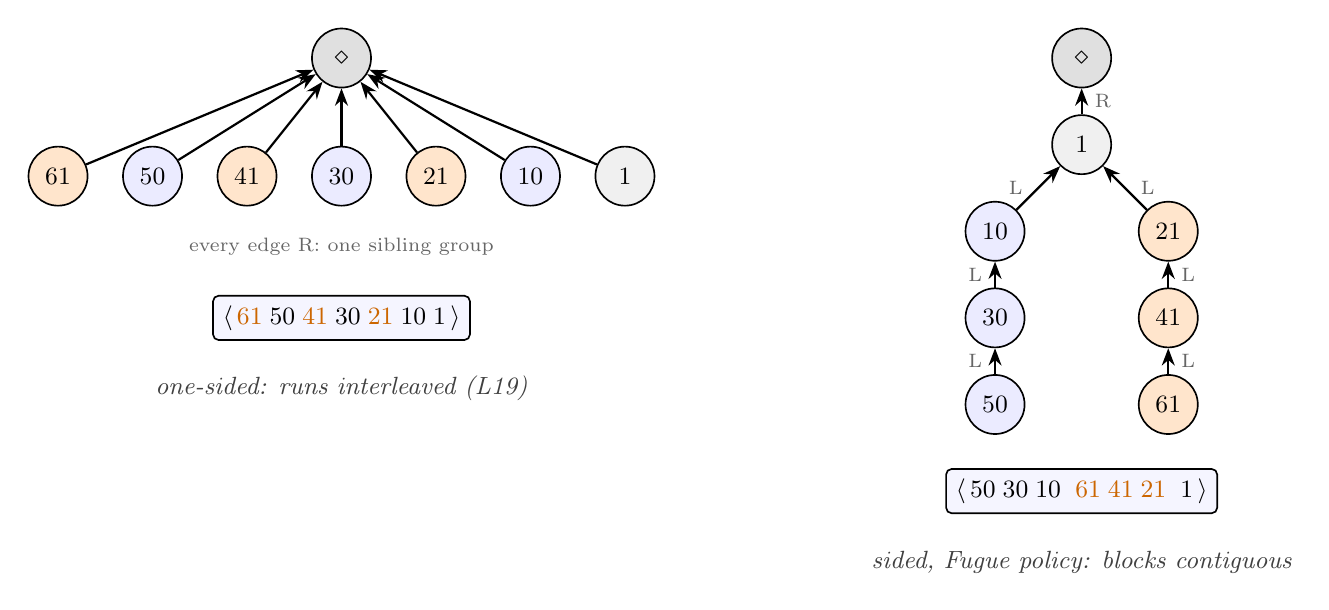
\begin{tikzpicture}
  % ---- left: one-sided (all-R), the L19 sibling fan
  \node[rootvtx] (fr) at (0,0) {$\diamond$};
  \node[vtx, fill=orange!20] (f61) at (-3.6,-1.5) {\small$61$};
  \node[vtx]                 (f50) at (-2.4,-1.5) {\small$50$};
  \node[vtx, fill=orange!20] (f41) at (-1.2,-1.5) {\small$41$};
  \node[vtx]                 (f30) at ( 0.0,-1.5) {\small$30$};
  \node[vtx, fill=orange!20] (f21) at ( 1.2,-1.5) {\small$21$};
  \node[vtx]                 (f10) at ( 2.4,-1.5) {\small$10$};
  \node[vtx, fill=black!6]   (f1)  at ( 3.6,-1.5) {\small$1$};
  \foreach \n in {f61,f50,f41,f30,f21,f10,f1}
    \draw[anc] (\n) -- (fr);
  \node[elbl] at (0,-2.4) {every edge R: one sibling group};
  \node[stbox] at (0,-3.3)
    {$\langle\,\textcolor{orange!80!black}{61}\;50\;
      \textcolor{orange!80!black}{41}\;30\;
      \textcolor{orange!80!black}{21}\;10\;1\,\rangle$};
  \node[capt] at (0,-4.2) {one-sided: runs interleaved (L19)};
  % ---- right: sided under the Fugue policy, backward runs = L-chains
  \begin{scope}[shift={(9.4,0)}]
  \node[rootvtx] (sr) at (0,0) {$\diamond$};
  \node[vtx, fill=black!6] (s1) at (0,-1.1) {\small$1$};
  \node[vtx]                 (s10) at (-1.1,-2.2) {\small$10$};
  \node[vtx, fill=orange!20] (s21) at ( 1.1,-2.2) {\small$21$};
  \node[vtx]                 (s30) at (-1.1,-3.3) {\small$30$};
  \node[vtx, fill=orange!20] (s41) at ( 1.1,-3.3) {\small$41$};
  \node[vtx]                 (s50) at (-1.1,-4.4) {\small$50$};
  \node[vtx, fill=orange!20] (s61) at ( 1.1,-4.4) {\small$61$};
  \draw[anc] (s1)  -- (sr) node[elbl, midway, right=1pt] {R};
  \draw[anc] (s10) -- (s1) node[elbl, midway, left=2pt]  {L};
  \draw[anc] (s21) -- (s1) node[elbl, midway, right=2pt] {L};
  \draw[anc] (s30) -- (s10) node[elbl, midway, left=1pt]  {L};
  \draw[anc] (s41) -- (s21) node[elbl, midway, right=1pt] {L};
  \draw[anc] (s50) -- (s30) node[elbl, midway, left=1pt]  {L};
  \draw[anc] (s61) -- (s41) node[elbl, midway, right=1pt] {L};
  \node[stbox] at (0,-5.5)
    {$\langle\,50\;30\;10\;\;
      \textcolor{orange!80!black}{61\;41\;21}\;\;1\,\rangle$};
  \node[capt] at (0,-6.4) {sided, Fugue policy: blocks contiguous};
  \end{scope}
\end{tikzpicture}
\caption{L19 under the two anchoring rules, the battery's own trace.
LCA document $\langle 1\rangle$; replica A (blue) types backward
$10, 30, 50$ before the head while replica B (orange) concurrently
types backward $21, 41, 61$. One-sided (left): every insert-before
anchors at the same left neighbor $\diamond$, both runs land in one
R-sibling group, and the timestamp-sorted fan interleaves them. Sided
under the Fugue policy (right): insert-before anchors at the
\emph{successor} as an L-entry, each run is an L-chain hanging off
$1$, and the in-order read keeps the blocks contiguous: L-extensions
precede the node ($50, 30, 10$ before their parents' line ending at
$1$), and among the L-siblings $10, 21$ of node $1$ the older run
displays first (the L band is mirrored). Both display strips are
machine outputs of \code{embed\_sided.py}.}
\label{fig:sided-l19}
\end{figure}

\paragraph{How the encoding realizes it, for zero extra bits.} The
one-sided block of \S\ref{sec:encoding} spends a constant leading
\code{1} per level whose only job is keeping coordinates nonempty;
repurpose it as the side bit. The L band needs an
order-\emph{reversing} prefix-free code, and the bit complement
$\overline{C}$ is exactly that at identical lengths (flipping every
bit flips every first-difference verdict and preserves both lengths
and prefix relations), so the block becomes
\[
  \mathrm{block}(\mathrm{side}, \delta) \;=\; \mathrm{sideBit}
  \,\|\, \bigl(C(\delta) \text{ if } R,\ \overline{C(\delta)}
  \text{ if } L\bigr),
\]
prefix-free per band, with no framing change and no new bits. On the
example, with the binary delta code ($C(1) = \code{0}$, $C(9) =
\code{1110001}$, $C(20) = \code{111100100}$, so $\overline{C(9)} =
\code{0001110}$, $\overline{C(20)} = \code{000011011}$), the stored
coordinates are the concatenated blocks:
\begin{center}\small
\begin{tabular}{@{}lll@{}}
\toprule
node & chain & stored coordinate (side bits marked) \\
\midrule
$1$  & $(R,1)$ &
  $\underline{\code{1}}\code{0}$ \\
$10$ & $(R,1)(L,9)$ &
  $\underline{\code{1}}\code{0}\;\underline{\code{0}}\code{0001110}$ \\
$21$ & $(R,1)(L,20)$ &
  $\underline{\code{1}}\code{0}\;\underline{\code{0}}\code{000011011}$ \\
$30$ & $(R,1)(L,9)(L,20)$ &
  $\underline{\code{1}}\code{0}\;\underline{\code{0}}\code{0001110}\;
   \underline{\code{0}}\code{000011011}$ \\
$50$ & $(R,1)(L,9)(L,20)(L,20)$ &
  $\underline{\code{1}}\code{0}\;\underline{\code{0}}\code{0001110}\;
   \underline{\code{0}}\code{000011011}\;
   \underline{\code{0}}\code{000011011}$ \\
\bottomrule
\end{tabular}
\end{center}
To compare two coordinates, parse: read a side bit; if \code{1},
decode one $C$ codeword as an R-band symbol $(R,\delta)$; if \code{0},
decode one $\overline{C}$ codeword (decode $C$ on the flipped bits) as
an L-band symbol $(L,\delta)$; repeat, then terminate with the marker.
Prefix-freedom per band delimits every block, so no length fields or
framing are needed, exactly as one-sided. The complement is what makes
the mirror free: within the L band, plain descending comparison of the
\emph{stored} bits is already the mirrored delta order ($
\overline{C(20)} = \code{000011011} < \overline{C(9)} = \code{0001110}
$ bitwise, matching $(L,20) < (L,9)$), so the carrier stores entropy
payload only and the marker-lex of the previous paragraph is read off
the bits. Faithfulness of this parse (unique decodability plus order
embedding of the sided alphabet) is machine-checked by the
chain-model/code-model lockstep below.

Two honest cost notes. Runs absorb the side bit like every other
run-constant (paid once at the head). On \emph{this} trace the sided
coordinates are longer than the one-sided fan's (the runs' deltas are
$20$ because the two replicas' Lamport clocks interleave); the
compression claim is about the common case, continuation-stamped
backward typing ($\delta = 1$ per keystroke, an \code{0}$\|
\overline{C(1)} = \code{01}$ block per level), where today's design
pays a growing-$\delta$ fan. Two-sidedness buys the semantics always
and the compression exactly when backward runs are locally stamped.

\paragraph{Side selection is a generation policy, not a datatype
choice.} If insert merely ``takes a side,'' convergence and
RA-linearizability hold for any sides whatsoever: those proofs never
consult the order's intent. What depends on \emph{which} side is
picked is the ordering intent. Fugue's non-interleaving needs the rule
``right child of the left neighbor when it has no right children, else
left child of the successor,'' and that rule lives at generation time,
where the framework already has a slot: honesty, the same layer that
polices the mint. The architecture is therefore one sided datatype,
verified once, policy-free (canonicity, fold exactness, the Join,
RA-linearizability), with intent theorems per generation policy: under
always-R, read-equivalence to the published RGA (the fragment theorem
composed with the compaction theorem); under the Fugue rule,
non-interleaving (a subtree is an in-order interval). RGA and Fugue
become two disciplines over one kernel rather than two datatypes.

\paragraph{Validation.} \code{whiteboard/litmus/embed\_sided.py}: the
chain semantics and the bit carrier as lockstep twin models, both run
under both policies. Every design prediction survived the first full
run:

\begin{center}\small
\begin{tabular}{@{}ll@{}}
\toprule
check & verdict \\
\midrule
full gauntlet under the Fugue policy (L1--L25, credential & clean,
  \textbf{including L19} \\
\quad family, subordination CEs, stale forks) &
  (out $= \langle 50,30,10,61,41,21,1\rangle$) \\
same gauntlet under always-R & clean except L19: the \\
 & one-sided fan, reproduced \\
chain semantics $\sim$ bit carrier, both policies & lockstep-EXACT
  (unique \\
 & decodability + order embedding) \\
all-R fragment $\sim$ the one-sided embed model & lockstep-EXACT, every
  scenario \\
randomized version-DAG PBT, all four models & 120 + 300 clean \\
\bottomrule
\end{tabular}
\end{center}

\noindent The Lean mechanization of both layers (the sided chain-lex
kernel and the sided conditioned instance, capstone included) has
landed kernel-clean; \S\ref{sec:mechanization} records it.

\section{Comparison with Eg-walker}
\label{sec:egwalker}

Eg-walker (Gentle \& Kleppmann, EuroSys 2025) is the closest system in
spirit, and the two designs can be read as the \emph{operational} and
\emph{denotational} realizations of one thesis, \textbf{pay for
concurrency, not for history}:

\begin{center}\small
\begin{tabular}{@{}p{0.31\textwidth}p{0.31\textwidth}p{0.31\textwidth}@{}}
\toprule
 & Eg-walker & embedded-chain RGA \\
\midrule
model & op-based; replicas exchange events & MRDT: three-way merge
  with an LCA \\
durable state & \textbf{full event graph on disk}, deletes included,
  retained while concurrent ops may arrive; document state
  metadata-free & \textbf{live nodes only}; no event log anywhere;
  dead survive as $\Theta(\log\delta)$ bits inside live coordinates \\
merge mechanism & \emph{replay}: walk the event graph, rebuild a
  transient CRDT structure (tombstones reappear transiently), discard
  at causally-linear points & \emph{refold}: $O(\text{survivors})$
  coordinate recomputation; no replay, no transient structure, no
  order decisions \\
sequential-editing cost & $\approx$ zero (plain edits; no metadata) &
  $\approx$ zero order metadata ($\sim$4 bits/level for continuation
  typing; a cursor jump pays log-gap once, at the run head) \\
concurrency cost & replay time proportional to the concurrent region,
  at every affected merge & coordinate bits proportional to
  $\log(\text{ts gap})$, once, in space \\
ordering semantics & Yjs-variant (FugueMax-adjacent); maximal
  non-interleaving \emph{conjectured}, not proved; two-sided (no L19
  analogue) & $\equiv$ published RGA (machine lockstep); one-sided:
  L19 backward-run interleaving inherited; removed by the sided
  generalization (\S\ref{sec:sided}), RGA kept as the all-R
  fragment \\
correctness artifact & informal proof (Appendix C) + property testing
  & L1--L25 battery + DAG PBT + lockstep vs RGA$_\dagger$;
  \textbf{RA-linearizability kernel-checked in Lean}
  (\S\ref{sec:mechanization}); the design was
  chosen so the merge proves itself (no order decisions to verify) \\
op payload & integer origin positions (compact, human-meaningful) &
  two timestamps + ghost prefix (droppable on the wire;
  \S\ref{sec:prefix}) \\
\bottomrule
\end{tabular}
\end{center}

\noindent Four sentences of honest positioning. \emph{(i)} Eg-walker
achieves its clean document state by keeping the entire history and
re-deriving order on demand; the embedded-chain RGA achieves it by
making order derivation unnecessary: the sort keys are written at
birth and never edited, and the coordinates are their encoding
(\S\ref{sec:encoding}), precomputed at mint time and exact forever.
\emph{(ii)} Eg-walker's ordering target was stronger where L19 is
concerned (Fugue-style two-sidedness removes backward interleaving,
while the one-sided design inherits RGA's anomaly by construction,
being read-equal to RGA); the sided generalization of
\S\ref{sec:sided} adopts exactly that two-sidedness as a parameter,
closing the gap while keeping the one-sided datatype as its all-R
fragment. \emph{(iii)} The verification gap runs
the other way: Eg-walker's replay-transform-clear loop is
algorithmically sophisticated and only informally proved; here the
merge performs no arbitration at all, the metatheory is one-line at
the chain layer plus a single faithfulness theorem at the encoding
layer, and RA-linearizability is a kernel-checked theorem in a
framework that had already verified a dozen-plus replicated
datatypes end-to-end (\S\ref{sec:mechanization}). \emph{(iv)} The
cost models part company at cursor jumps: a single-user history that
hops back to type at an old anchor is free for Eg-walker (nothing
concurrent to replay) but mints log-gap bits here, once per jump, at
the run head; on measured single-user editing traces the jump tail
is thin (code bits $\approx 1.4$--$1.8$ per level; see the companion
note of \S\ref{sec:encoding}). In the MRDT setting there is also a model
fit: Eg-walker must reconstruct merge context by replay because the
op-based model gives it none; the MRDT model hands the merge its LCA,
which is exactly the context replay rebuilds.

\section{Related work}
\label{sec:related}

The verified sweep of nearby systems lives in
\code{whiteboard/litmus/related-work.md} (per-claim verdicts, primary
sources); this section positions the datatype.

\paragraph{Retention taxonomy.} What nearby systems keep for the dead:
tombstone records (RGA with cemetery under causal stability; WOOT;
Yjs's per-deletion GC structs, kept forever; Fugue, ``we cannot
remove a deleted element's node entirely''; Peritext, ``the
positions must be remembered''); the full history (Eg-walker's event
graph, Chronofold/causal trees where the log \emph{is} the text);
consensus-gated compaction (Treedoc's flatten requires Paxos-commit);
or \textbf{dead identifiers inside live position keys} (Logoot/LSEQ,
Weidner's position-strings/list-positions, the Fugue id space). The
embedded-chain RGA is in the last class \emph{by information content}
(dead ancestors' timestamps persist inside survivors' sort keys,
at live-reachable scope), but with three deltas to its classmates:
the retention is \emph{delta-coded at the entropy of the anchor
gaps} (a sequential
history costs a constant per element where Logoot-family keys grow
with allocation policy), the \emph{birth tree kept whole} gives
forward non-interleaving and delete-order preservation (position-key
designs interleave, the PaPoC'19 anomaly, and Figma-style
fractional indexing is unsound under concurrency by its own account),
and the semantics is pinned to the best-studied sequence CRDT by a
machine-checked lockstep rather than being a new point in anomaly
space.

\paragraph{The impossibility backdrop.} Attiya et al.\ (PODC 2016)
prove $\Omega(D)$ metadata for push-based protocols meeting even the
weak list spec: the published form of ``ordering requires
remembering the dead.'' This design does not escape the bound; it
\emph{relocates and minimizes} the memory: $\Theta(\log \delta)$ bits
per dead-chain element inside live coordinates (plus the MRDT version
store, which the model provides). The sharper, machine-witnessed
form from our design sweep is the \emph{conservation law}
(\S\ref{sec:design}):
the sort key must retain dead ancestors' timestamps (the verdict
information survives every encoding change: stamp, spine, tombstone,
or denominator bits), and ties force separate \emph{metadata} only
under timestamp-oblivious minting; the timestamp-faithful mint carries
the same bits inside the coordinate. Eight timestamp-oblivious
mutation variants each have a named machine-checked countermodel
(fold-verdict erasure; repair non-locality); the credential
countermodel separates this design from all of them.

\paragraph{Verified datatypes.} Isabelle RGA (Gomes et al.\ OOPSLA'17,
op-based convergence), OpSets (list semantics specified by a total
order of identified ops: arbitration-by-identity as specification),
VeriFx (SMT, convergence properties), MET (TLA+, list CRDT bugs). In
the MRDT line (Kaki et al.\ OOPSLA'19; Peepul PLDI'22; RA-lin
OOPSLA'25, this framework), no verified sequence with
sequence-CRDT-grade ordering guarantees exists; our verified rehoming
RGA (\S\ref{sec:design}) is RA-linearizable against its own fold yet
fails the sequential delete-order spec, since RA-linearizability
certifies convergence to the datatype's \emph{own} semantics and
ordering intent must be specified and proved separately. The
embedded-chain RGA delivers the missing artifact:
RA-linearizability is a kernel-checked Lean theorem
(\S\ref{sec:mechanization}); delete-order preservation, display
stability and forward non-interleaving are proved at the model layer;
and the RGA read-equivalence (the compaction theorem,
\S\ref{sec:mechanization}) closes the intent question against the
best-studied sequence semantics.

\paragraph{Treedoc's lesson, inverted.} Treedoc re-balances geometry
and must pay consensus for it; the principle that emerged from our
ledger-based sibling design study
(\emph{reprojection without consensus is safe iff geometry has been
demoted to a rendering}) is here taken to its fixed point: geometry is
never reprojected at all. It is immutable, so it may safely be the
only thing.

\section{Mechanization status}
\label{sec:mechanization}

The verification framework is the RA-linearizability metatheory for
MRDTs (OOPSLA'25), mechanized in the Sal Lean development, the
same framework in which twelve production MRDTs (the rehoming RGA
among them) and a further half-dozen born-conditioned instances (the
Peepul mergeable queue included) are verified end-to-end; file paths
below are relative to that repository.

\textbf{The capstone is proved} (2026-07-15, kernel-clean on
$\{\mathrm{propext}, \mathrm{Classical.choice},
\mathrm{Quot.sound}\}$):
\[
  \code{embed\_ra\_linearizable3} \;:\;
  \mathrm{EReach}\ \Gamma\ C \to \mathrm{IsRALinearizable3}\ C
\]
i.e.\ RA-linearizability per version at every honestly reachable
configuration, \emph{parametric in the code} $\Gamma$: the unary
code, the binary delta code, and the flipped Elias-$\delta$ code are
all proved \code{OrderedPrefixCode} instances, three encodings on
one proof. The factoring is exactly this
note's design--encoding split, which is itself evidence for the split:

\begin{enumerate}
\item \textbf{Model layer} (\code{Sal/MRDTs/RGA\_Embed/}, six
files, 0 sorry, plus the read-equivalence order core and the sided
kernel noted below): the code-parametric kernel; commutations \emph{to
state equality} under $\rc = \Either$ (\code{rc\_non\_comm'});
\code{ins\_prefix\_ghost}; coherence and chain-generation closures;
display stability, with step stability (S2, delete-order preservation at
its `del` instance) proved \emph{without any axioms} and merge pairwise
stability (S4, the adopted contract); unique decodability
(\code{coordOf\_inj}); \textbf{the chain-lex theorem}
(\code{display\_iff\_chainBefore} = Corollary~\ref{cor:lex});
non-interleaving as subtree convexity (\code{subtree\_convex});
Theorem~\ref{thm:faithful}(i) for all three codes
(\code{binEnc\_mono}/\code{binEnc\_prefixFree},
\code{dEnc\_mono}/\code{dEnc\_prefixFree}, cross-validated
against the Python codes by kernel \code{decide});
\code{native\_decide} SPOTs where the rehoming RGA's delete-reorder
witness gets the opposite verdict.
\item \textbf{Conditioned instance}
(\code{Sal/ConditionedMRDTs/MRDT\_Instances/EmbedRGA/}, nine
sections, 0 sorry, plus the Elias-$\delta$ inheritance corollary
\code{EmbedRGA\_EliasDelta.lean}), proved via the \emph{mergeable-queue route}: a
generic join lemma (\code{JoinLemma3At}: the merge exhibits its own
linearization witness) plus an honest-reachability metatheorem
(\code{HonestReach}), rather than the rehoming RGA's 55-file bespoke
chain. The route applies exactly when states are canonical per event
set, which is Theorem~\ref{thm:chain}(i).
Landed: the canonical sorted-list state; strictly-sorted
extensionality (\code{esorted\_ext}: sorted lists with the same
members are equal, replacing any canonical-list formula);
\textbf{fold-canonicity} (\code{e\_fold\_canon}: well-formed
enumerations of one event set fold to the \emph{same} state;
Theorem~\ref{thm:chain}(i) mechanized); the honesty core and its
bridge to well-formedness; the merge membership characterization
(\code{e\_mergeL\_mem}, OR-set survival with honesty closing the
cross-branch-delete corner); the Join (\code{e\_join\_at}: the
merge is its own linearization witness); the capstone; the honesty
discharge from the framework's generation discipline
(\code{eHonest\_of\_applicable}: applicable generation forces the
honesty core, so per-op honesty needs no bespoke oracle); and the
instance intent theorems: delete-order preservation \emph{is}
sublist stability (\code{eUpdate\_del\_sublist} is literally
\code{List.filter\_sublist}: a delete's successor state is a sublist
of its predecessor, so the surviving display order is untouched;
the merge preserves each input's survivor order on both sides).
\end{enumerate}

\noindent\textbf{The compaction theorem is proved} (2026-07-15,
kernel-clean): $\mathrm{read} \circ \mathrm{embed} = \mathrm{read}
\circ \mathrm{RGA}_\dagger$ on honest executions, as
\code{rga\_read\_eq\_embed\_read}
(\code{EmbedRGA\_ReadEquiv.lean}): for every well-formed enumeration
of an honest event set, \emph{any} enumeration of the tombstoned
fold's visible ids in the published RGA's own relational order
(\code{visible\_lt}) equals the embed fold's id sequence, with
element agreement (\code{embed\_rec\_readSeq}). The proof is
\emph{against the published definition}: the order core
(\code{Sal/MRDTs/RGA\_Embed/RGA\_Embed\_ReadEquiv.lean}) shows
\code{visible\_lt} coincides with chain-lex on the shared birth tree
(soundness by induction on derivations, completeness by realizing
every chain prefix as an \code{afters}-reachable ancestor), and en
route proves the published relational order total and asymmetric on
the birth tree, facts the published side never had. This converts
the design into a theorem \emph{about} the published RGA: it admits a
strictly-live compaction preserving every read. The lockstep rows of
\S\ref{sec:validation} are this theorem's tested form.

\medskip
\noindent\textbf{The sequential specification is proved, and the
design now holds the canonical seat} (2026-07-16). The
sequential-specification campaign (its self-contained note:
\code{Sal/ConditionedMRDTs/seqspec-campaign.pdf}) proved
\code{embed\_seq\_sound}: on every sequentially honest single-replica
history the canonical sorted state IS the naive insert-at-position
text buffer, record for record, with the adjacency lemma
(\code{chainBefore\_snoc\_iff}: a fresh insert's delta beats every
existing child's by sum-telescoping) as the geometric heart; the
published RGA$_\dagger$ inherits the same buffer spec through the
compaction theorem (\code{rga\_seq\_read\_eq\_buffer}). The same
statement is REFUTED for the rehoming design
(\code{rehoming\_seq\_refuted}: the \S\ref{sec:validation} L1 row
generalized to a kernel-checked refutation on an honest four-op
trace), which demoted it repo-wide: the embedded-chain family is now
the repository's canonical sequence RDT, and the canonical fused
Peritext was re-based onto THIS kernel
(\code{Peritext\_Embed/}: capstone by pure instantiation of the
payload-generic instance; \code{renderIds\_del}, deleting a character
never re-formats another, the theorem the rehoming kernel provably
lacks; and the tier-4 editor theorem
\code{peritextEmbed\_seq\_sound}). One caveat is recorded as an open
question (oq:seqwitness, campaign note \S8): per-replica soundness
and convergence do not compose into ``the merged read is the naive
buffer on some ordering of the union''; the dead-anchor corner is
where stamp-sorted replay diverges from the fold.

\medskip
\noindent\textbf{The sided generalization is proved} (2026-07-15,
kernel-clean), in the same two layers as \S\ref{sec:sided} presents
it. The sided chain-lex kernel
(\code{Sal/MRDTs/RGA\_Embed/Sided\_ChainLex.lean}): the sided marker
theorem \code{sdisplay\_iff\_schainBefore} (display comparison of
sided coordinates IS the in-order rule), totality of the display
relation \emph{without any axioms}, unique decodability
(\code{sidedCoordOf\_inj}: the side is recoverable from the first
symbol's band, the delta by prefix-freedom within the band), the
all-R \emph{fragment theorem} \code{schainBefore\_liftR} (all-R chains
order exactly as one-sided chains: ``RGA is the all-R fragment,''
mechanized), and in-order-interval subtree convexity
(\code{schain\_subtree\_convex}, the datatype half of the L19
discharge). The conditioned instance
(\code{MRDT\_Instances/SidedRGA/}, nine sections mirroring the
one-sided instance with the sided key): fold-canonicity
(\code{s\_fold\_canon}), the Join by the same mergeable-queue route,
and the capstone
\[
  \code{sided\_embed\_ra\_linearizable3} \;:\;
  \mathrm{SReach}\ \Gamma\ C \to \mathrm{IsRALinearizable3}\ C
\]
\emph{for every side assignment}: sides are payload to convergence,
which is the policy/datatype split of \S\ref{sec:sided} as a theorem,
with \code{sHonest\_of\_applicable} discharging honesty from the
generation guard exactly as one-sided. The per-policy intent
theorems have since landed, and the policy story is a machine-checked
three-act arc (2026-07-16/17). \emph{Act one}: \code{sFold\_liftOp},
the all-R sided fold IS the one-sided fold, unconditionally (the sort
keys coincide definitionally), so every one-sided theorem transports;
and \code{sided\_fold\_subtree\_convex}, subtrees display as
contiguous blocks in any chain-generated fold, so runs that chain
never interleave (\code{fugue\_reachable\_runs\_no\_interleave}).
\emph{Act two}: the Weidner--Kleppmann maximal-non-interleaving
Definition~4 was formalized over reachable configurations
(\code{SidedRGA\_Fugue.lean}) and REFUTED twice for this Fugue
policy on reachable traces (the recency tiebreak reverses the paper's
lowest-ID-first; their Figure-7 execution): the paper's own
Fugue-vs-FugueMax separation, landing on this implementation.
\emph{Act three}: FugueMax realized as a kernel variant
(\code{SidedMax\_ChainLex.lean}): its sibling order depends on the
right ORIGIN, not expressible by any re-banding of deltas (the mirror
control machine-witnesses this), so R-entries carry the mint-time
successor's key as an order-reversing tag; condition (3) is proved in
full (\code{fuguemax\_same\_origin\_low\_first}, the positive twin
of the refutation) and full Theorem~9 is reduced to exactly two
stated gaps, the display-to-traversal theory (task \#88). The sided
sequential spec also landed (\code{sided\_seq\_sound}: a
sentinel-rooted two-sided buffer, R-inserts splice after their
anchor, L-inserts immediately before). The tag has a COST: at
contested inserts the coordinate embeds the successor's key,
$\Theta(|\text{key}|)$ where plain Fugue pays zero, and whether that
retention is a lower bound for tombstone-free maximal
non-interleaving is an open question with a Myhill--Nerode shape
(task \#89): the entropy law of \S\ref{sec:encoding} meeting the
ordering intent.

\paragraph{Provenance.} \code{whiteboard/litmus/embed\_tree.py} (the
design, the timestamp-oblivious control, the credential countermodel,
the IEEE 754 measurements; \code{python3 embed\_tree.py} /
\code{fp} / \code{code}); \code{litmus.py}, \code{pbt.py} (battery and
DAG harness); \code{contest\_tree.py} (lockstep harness, CE
regressions); \code{whiteboard/retention-countermodel.pdf} (the
retention arc that forced this design);
\code{whiteboard/delta-tree-design.pdf} (the ledger-based sibling
design and the invariants I1--I3);
\code{whiteboard/litmus/related-work.md} (verified source list:
Roh et al.\ JPDC'11; Attiya et al.\ PODC'16; Kleppmann et al.\
PaPoC'19; Weidner \& Kleppmann TPDS'25 (Fugue); Gentle \& Kleppmann
EuroSys'25 (Eg-walker, arXiv:2409.14252); Preguiça et al.\ ICDCS'09
(Treedoc); Grishchenko \& Patrakeev PaPoC'20 (Chronofold); Litt et
al.\ CSCW'22 (Peritext); Gomes et al.\ OOPSLA'17; OpSets 2018; Kaki et
al.\ OOPSLA'19; Peepul PLDI'22; RA-lin OOPSLA'25; VeriFx ECOOP'23;
Figma/Wallace fractional indexing; Weidner position-strings).

\end{document}
